%%%%%%%%%%%%%%%%%%%%%%%%%%%%%%%%%%%%%%%%%%%%%%%%%%%%%%%%%%%%%%%%%%%%%%%
% Universidade Federal de Santa Catarina             
% Biblioteca Universitária                     
%----------------------------------------------------------------------
% Exemplo de utilização da documentclass ufscThesis
%----------------------------------------------------------------------                                                           
% (c)2013 Roberto Simoni (roberto.emc@gmail.com)
%         Carlos R Rocha (cticarlo@gmail.com)
%         Rafael M Casali (rafaelmcasali@yahoo.com.br)
%%%%%%%%%%%%%%%%%%%%%%%%%%%%%%%%%%%%%%%%%%%%%%%%%%%%%%%%%%%%%%%%%%%%%%%
\documentclass{ufsctex} % Definicao do documentclass ufscThesis	


%----------------------------------------------------------------------
% Pacotes usados especificamente neste documento
\usepackage{graphicx} % Possibilita o uso de figuras e gráficos
\usepackage{color}    % Possibilita o uso de cores no documento
\usepackage{pdfpages} % Possibilita a inclusão da ficha catalográfica
\usepackage{listings} % Possibilita colocar códigos
\usepackage{lipsum}
\usepackage{caption} % colocar textos em figuras
\captionsetup{justification=raggedright,singlelinecheck=false, labelsep=endash}%, textfont=footnotesize}
\usepackage{subfigure}
\usepackage{xifthen} % deixa fazer uns if-then-else mutcho loko
\usepackage[brazil]{babel}  % usados para arrumar os caracteres em português
\usepackage[utf8]{inputenx} % 
%\usepackage[utf8]{inputenc}
\usepackage[T1]{fontenc}    %
\usepackage{mathtools}
\usepackage{graphicx}
\usepackage{lmodern}
\usepackage{calc}
\usepackage{enumitem}
\usepackage{bibentry} % permite usar o comando nobibliography
\usepackage{minted} % Sintaxe colorida
\usepackage{booktabs}
\usepackage{xparse} % Permite definir umas funções com mais recursos.

%\usepackage[square,numbers]{natbib}
%----------------------------------------------------------------------
% comandos de customização dos pacotes
\renewcommand\listingscaption{Algoritmo}
% \renewcommand{\lstlistlistingname}{Lista de \lstlistingname s}% List of Listings -> List of Algorithms

\graphicspath{{figuras/}}


% Numeração das tabelas e figuras de acordo com o capítulo
\usepackage{amsmath}
\numberwithin{table}{chapter}
\numberwithin{figure}{chapter}

%----------------------------------------------------------------------
% Comandos criados pelo usuário
\newcommand{\afazer}[1]{{\color{red}{#1}}} % Para destacar uma parte a ser trabalhada
\newcommand{\ABNTbibliographyname}{REFERÊNCIAS} % Necessário para abnTeX 0.8.2

\newcommand{\figura}[5][Fonte:]{
	\begin{figure}[h!tb]
		\caption{#3.}
		\includegraphics[width=#4]{#2.png}
		\ifthenelse{\isempty{#5}}{}{%
			\\ \footnotesize{#1 \citeonline{#5}.}
		}	
		\label{fig:#2}
	\end{figure}
}

\NewDocumentEnvironment{tabela}{mm}
{
	\begin{table}[htb]
	
	{
	    %TODO: Rever
	}
		\caption{#2}
		\label{tab:#1}
	\end{table}
}

\newcommand{\reffig}[1]{Figura \ref{fig:#1}}
\newcommand{\refalg}[1]{Algoritmo \ref{alg:#1}}
\newcommand{\reftab}[1]{Tabela \ref{tab:#1}}
\newcommand{\refcap}[1]{\footnote{vide tópico \ref{cap:#1}.}}
\newcommand{\reftop}[1]{Seção \ref{cap:#1}}

\newcommand{\criarSigla}[3][]{%
	\ifthenelse{\isempty{#1}}{%
		#2 (#3)\sigla{#3}{#2}%
	}{%
		\emph{#2} (#3)\sigla{#3}{\emph{#2}}\footnote{Traduzido como: #1.}%
	}%
}

%----------------------------------------------------------------------

%----------------------------------------------------------------------
% Identificadores do trabalho
% Usados para preencher os elementos pré-textuais
\instituicao[a]{Universidade Federal de Santa Catarina} % Opcional
\departamento[a]{Departamento de Computação} %TODO departamento de engenharia da computação?
\curso[a]{Universidade Federal de Santa Catarina}
\documento[o]{Trabalho\ de\ Conclusão\ de\ Curso} % [o] para dissertação [a] para tese

\titulo{Um modelo de geladeira aprimorado que facilite a vida dos usuários e que leva em conta suas preferências}

%\subtitulo{Subtítulo} % Opcional


\autor{Thiago Raulino Dal Pont}
\grau{Bacharel em Engenharia de Computação}
\local{Araranguá} % Opcional (Florianópolis é o padrão)
\data{04}{dezembro}{2017}
\coordenador[Coordenadora]{Prof. Dr. Eliane Pozzebon} %TODO Rever o Coordenador do curso
\orientador[Orientador]{Prof. Dr. Alexandre Leopoldo Gonçalves}
%\coorientador[Coorientador\\Universidade ...]{Prof. Dr.}

\numerodemembrosnabanca{3} % Isso decide se haverá uma folha adicional
\orientadornabanca{sim} % Se faz parte da banca definir como sim
\coorientadornabanca{não} % Se faz parte da banca definir como sim
\bancaMembroA{Primeiro membro\\Universidade ...} %Nome do presidente da banca
\bancaMembroB{Segundo membro\\Universidade ...}      % Nome do membro da Banca
\bancaMembroC{Terceiro membro\\Universidade ...}     % Nome do membro da Banca
\bancaMembroD{Quarto membro\\Universidade ...}       % Nome do membro da Banca
%\bancaMembroE{Quinto membro\\Universidade ...}       % Nome do membro da Banca
%\bancaMembroF{Sexto membro\\Universidade ...}        % Nome do membro da Banca
%\bancaMembroG{Sétimo membro\\Universidade ...}       % Nome do membro da Banca

\dedicatoria{Dedico este trabalho aos meus pais e meu irmão, sem os quais jamais chegaria até aqui, e a todos os colegas e professores que me guiaram ao longo do curso.}

\agradecimento{A todos qυе direta оυ indiretamente fizeram parte dа minha formação, о mеυ muito obrigado.}

\epigrafe{Se A é o sucesso, então A é igual a X mais Y mais Z. O trabalho é X; Y é o lazer; e Z é manter a boca fechada.}


	%}



\textoResumo {
%Introdução e contextualização
Nas últimas duas décadas o conceito de Internet das Coisas vem se popularizando, propondo a introdução da tecnologia e da interconexão de objetos distintos, como lâmpadas, geladeiras, carros, etc., através de uma rede, frequentemente, a Internet. Assim, o número de aparelhos interligados tende a crescer produzindo uma grande quantidade de dados. Torna-se, então, necessário o uso de ferramentas capazes de processar e extrair informações relevantes desses dados. Entre os métodos existentes estão os sistemas de recomendação, aos quais, a partir de análises da interações de usuários, são capazes de traçar perfis de usuários e fornecer sugestões. Nos últimos anos, esses sistemas vêm sendo incorporados em diversos contextos como plataformas de \textit{streaming} e, gradativamente, outras aplicações introduzirão tais ideias no âmbito da Internet das Coisas. Entre os ambientes, nos quais é possível integrar ambos os conceitos, estão as casas inteligentes ou \textit{smart homes}, onde o uso da tecnologia abre caminho para novas formas de interação com o lar. Dispositivos comuns presentes em casas, como geladeiras, agregam, assim, novas tecnologias e funcionalidades, no entanto, os modelos existentes apenas proporcionam interações digitais, contudo não atentam aos gostos e hábitos dos usuários. Levando isso em conta, o presente trabalho propõe um modelo de geladeira capaz de monitorar as interações e traçar perfil de preferências por produtos. Isso é possível devido ao uso de etiquetas RFID, que terão o papel de identificar os diversos produtos contidos na geladeira e da aplicação de algoritmos de recomendação. Ao final, fez-se uma avaliação, a partir de um cenário criado, onde o equipamento foi capaz de realizar o monitoramento dos produtos disponíveis e de oferecer recomendações aos usuários a partir o seus perfis, além da reposição de produtos considerados essenciais. Além disso, foi possível recomendar receitas tanto a partir do conteúdo da geladeira, bem como, do perfil do usuário. A partir do exposto, conclui-se que a integração dos conceitos de Internet das Coisas e Sistemas de Recomendação pode contribuir para auxiliar usuários em suas tarefas diárias facilitando, de algum modo, o processo de tomada de decisão.}

% Ao final, o equipamento será capaz de oferecer novos produtos ao usuário de acordo com o seu perfil, além de promoções de itens relacionados e sugestões de receitas que englobem produtos contidos na geladeira.

% Ao final, o equipamento foi capaz de oferecer novos produtos ao usuário, a partir o seu perfil, além da reposição de  produtos considerados essenciais. Além disso, foi possível recomendar receitas tanto a partir do conteúdo da geladeira, bem como, do perfil de preferências do usuario.

\palavrasChave {Internet das Coisas. Sistemas de Recomendação. Geladeira Inteligente. Preferências do usuário.}

% No final vai ter 4 PARTES: 

% Introdução / cont
% materiais e métodos
% resultados alcançados
% conclusões

% TCC 1 
% Introdução / cont
% materiais e métodos
% resultados esperados


% Nas últimas duas décadas o paradigma da Internet das Coisas vem emergindo, propondo a introdução da tecnologia e da inter-conexão de objetos distintos como lâmpadas, geladeiras, carros, etc., através de uma rede, sendo esta, muitas vezes, a Internet. Além disso, com o grande número de aparelhos interligados, se produzirá altas quantidades de dados provenientes das interações com o ambiente e com os usuários. Assim, torna-se necessário o uso de ferramentas que processem e extraiam informações relevantes desses dados. Entre os métodos existentes estão os sistemas de recomendação, aos quais, a partir da análise dos registros das interações, são capazes de traçar o perfil de usuários. Nos últimos anos, esses sistemas vêm sendo aplicados em diversos contextos como plataformas de \textit{streaming}.  O presente trabalho propõe um novo modelo de interação entre geladeiras e usuários, onde o equipamento a partir dos algoritmos citados é capaz de monitorar as interação com o usuário e a traçar o seu perfil de preferências em produtos. Isso é possível graças ao uso etiquetas RFID, aos quais operam por radio frequência, que terão o papel de identificar os diversos produtos contidos na geladeira e as interações do usuário com tais produtos. A partir disso é possível traçar um perfil do usuário a partir de algoritmos de recomendação. Ao final, a geladeira será capaz de oferecer novos produtos ao usuário de acordo com o seu perfil além de promoções. É possível que o usuário selecione um conjunto de produtos essenciais, ou seja, que jamais podem faltar e a partir disso realizar compras automáticas. A partir do perfil, será possível também fazer sugestões de receitas que englobem os produtos contidos na geladeira.
\textAbstract {In the last two decades the concept of the Internet of Things has become popular, proposing the introduction of technology and the interconnection of different objects such as lamps, refrigerators, cars, etc. through a network, often the Internet. Thus, the number of interconnected devices tends to grow and high amounts of data will be produced. It is then necessary to use tools capable of processing and extracting relevant information from this data. Among the existing methods are the recommendation systems, which, from the analysis of the records, are able to trace the users profile and provide suggestions. In recent years, these systems have been incorporated in a variety of contexts as streaming platforms and, gradually, applications will introduce these ideas into the Internet of Things. Among the environments in which both concepts can be integrated are smart houses, where the use of technology opens the way to new forms of interaction with the home. Common devices such as refrigerators add technologies and new features, however, the existing models only provide digital interactions, however do not pay attention to the tastes and habits of users. Taking this into account, the present work proposes a new refrigerator model capable of monitoring interactions and tracing preferences profile in products. This is possible thanks to the use of RFID tags, which will have the role of identifying the various products contained in the refrigerator and the application of recommendation algorithms. In the end, the equipment will be able to offer new products to the user according to their profile, as well as promotions of related items and suggestions of recipes that include products contained in the refrigerator}
\keywords {Internet of Things. Recommender systems. Smart fridge. User preferences}



%----------------------------------------------------------------------
% Início do documento                                
\begin{document}
	%--------------------------------------------------------
	% Elementos pré-textuais
	\capa  
	%\folhaderosto[comficha] % Se nao quiser imprimir a ficha, é só não usar o parâmetro
	
	\begin{titlepage}
	\vfill
	\begin{center}
		%{\large \ABNTautordata} \\[5cm]
		\ABNTautordata \\[5cm]
		
		\tituloformat{\ABNTtitulodata}: \\
		\tituloformat{\subtitulodata} \\[1cm]
		
		\hspace{.45\textwidth} % posicionando a minipage
		\begin{minipage}{.5\textwidth}
			\begin{espacosimples}
				
				Trabalho de Conclusão de Curso submetido à \ABNTinstituicaodata,
				como parte dos requisitos necessários para a obtenção do Grau de
				Bacharel em Engenharia de Computação.
				
				Orientador: Prof. Alexandre Leopoldo Gonçalves, Dr.
			\end{espacosimples}
		\end{minipage}
		\vfill \localformat \ABNTlocaldata, \mesdata\ de \anodata.
	\end{center}
	\vspace{1cm}
\end{titlepage}



	
	% \folhaaprovacao
	% \paginadedicatoria
	% \paginaagradecimento
%	\paginaepigrafe
	\paginaresumo
	\paginaabstract
	%\pretextuais % Substitui todos os elementos pre-textuais acima
	\listadefiguras % as listas dependem da necessidade do usuário
	\listadetabelas 
	\listadeabreviaturas
	\listadesimbolos
	\sumario
	
	%--------------------------------------------------------
	% Simbolos e Abreviaturas
	%\abreviatura{RAM}{\emph{Random Access Memory}}
	\abreviatura{IoT}{\emph{Internet of Things}}
	\simbolo{$\int$}{Integral}
	
	%########################################################
	% Elementos textuais
	
	\chapter{Introdução}

Nas últimas décadas, presencia-se os acelerados avanços na ciência e tecnologia impulsionados por empresas dos mais diversos ramos e pelas constantes pesquisas nas universidades. 

Um dos avanços tecnológicos mais significativos é a Internet, com efeito significativo no desenvolvimento da economia global e na sociedade atual. Em duas décadas tem decorrido um grande crescimento na disponibilidade do acesso à rede. Em setembro de 2016, o número de usuários da rede mundial de computadores era de aproximadamente 3,75 bilhões, quase metade da população mundial e cerca de 92 vezes maior em relação ao ano 2000 \cite{MiniwattsMarketingGroup2016}.  Outro grande avanço tem ocorrido nos celulares, aos quais evoluíram tanto nos últimos anos que passaram de simples e grandes telefones sem fio à dispositivos menores, no entanto, com acesso à Internet, recursos avançados de áudio e vídeo e poder de processamento equiparável à computadores de mesa (\textit{desktops}) e/ou notebooks \cite{Meyers2011, Woyke2014}.

Em meio ao contexto da Internet, um novo paradigma surgiu no meio acadêmico e aos poucos ganha terreno nas grandes empresas. A sua proposta é levar a tecnologia a objetos do dia a dia, como condicionadores de ar, lâmpadas, fogões etc., e, assim, criar novas formas de interação além de funcionalidades inéditas, seguindo o exemplo dos \textit{smartphones}. 


Mencionada pela primeira vez, por Kevin Ashton, em 1999 \cite{Finep2015}, a Internet das Coisas (IoT, do inglês, \textit{Internet of Things}) vem se consolidando cada vez mais. Abrigará um variado ecossistema de dispositivos com capacidade de processamento, sensoriamento, conexão com demais dispositivos, em muito casos, com a Internet, entre outros avanços. Estima-se que, em 2020, cerca de 24 bilhões de dispositivos IoT estejam conectados, implicando em torno de quatro dispositivos por pessoa \cite{Meola2016}.   
Contudo, com o crescimento do número de itens computacionais, a quantidade de dados gerada por eles também cresce de maneira acelerada \cite{Chiang2016}. A partir disso, o fluxo de dados na rede de internet se intensifica a ponto de comprometer o seu desempenho. Isso decorre do modelo de rede utilizado, também chamado \textit{cloud computing}, ao qual mantêm recursos e funcionalidades distantes dos dispositivos que os utilizam, ou seja, em servidores e \textit{data centers}. Assim, para obtenção de tais recursos há a necessidade dos dispositivos em acessar a nuvem através da internet sempre que necessário, gerando, desse modo, um alto tráfego de dados \cite{Vaquero2014}. 
Além disso, o acesso a nuvem dificulta aplicações em IoT em tempo real devido ao atraso entre envio e recebimento de dados pela rede de internet \cite{Syed2016}.
% original: Isso ocorre devido ao modelo atual de funcionamento da rede, ou seja, centralizado.
Portanto, uma nova arquitetura se faz necessária para incorporar os dispositivos IoT à Internet tradicional. 
Nesse contexto, a \textit{fog computing} ou computação de neblina, surge como potencial solução, com base na proposta de uma forma de organização de rede que complemente a atual. Isso é possível com base na aproximação, aos dispositivos IoT que as utilizam, de algumas funcionalidades e recursos que atualmente são acessados através da nuvem, ou seja, centralizadas em servidores e data centers.
% Original: Isso é possível com base na aproximação de algumas funcionalidades, centralizadas em servidores, aos dispositivos que as utilizam
\cite{Chiang2016}. Para tanto, um dispositivo de rede seria responsável por uma ``nuvem local'' ou \textit{fog}. Desse modo, os dispositivos IoT se comunicariam com esse equipamento e obteriam funcionalidades necessárias de maneira mais eficiente. Ademais, a nuvem local se comunicaria diretamente com a nuvem convencional, transferindo apenas informações mais relevantes e necessárias \cite{Syed2016}.

Os dispositivos que compõem a Internet das Coisas podem ser denominados objetos inteligentes, ou \textit{smart objects}, aos quais detêm funcionalidades expandidas como comunicação, sensoriamento, processamento e atuação sobre o ambiente. Além disso, promovem a interação entre o mundo físico (analógico) e o mundo digital. Isso ocorre graças a sensores capazes de capturar grandezas como temperatura e luminosidade e, a partir disso, torna-se possível que aplicações tenham conhecimento do contexto do ambiente \cite{Stojkoska2017}. 

Baseando-se nesses conceitos, algumas companhias vêm inserindo no mercado novos produtos com as características citadas. Como exemplo, é citável o Amazon Echo\textsuperscript{\textregistered}\footnote{https://www.amazon.com/Amazon-Echo-Bluetooth-Speaker-with-WiFi-Alexa/dp/B00X4WHP5E}, um dispositivo que opera com o serviço de assistente pessoal Alexa, e interage com pessoas em uma casa a partir de comando de voz. Outro produto destacável é a \textit{smart lock} da empresa Nuki\textsuperscript{\textregistered}\footnote{https://nuki.io/en/shop/nuki-smart-lock/}, pelo qual é possível abrir e fechar a porta apenas com um toque no aplicativo móvel pelo \textit{smartphone} ou através de um \textit{smart watch}. Ademais, outras áreas vem se utilizando desses conceitos, por exemplo, os esportes. O CARV\textsuperscript{\textregistered}\footnote{https://www.kickstarter.com/projects/333155164/carv-the-worlds-first-wearable-that-helps-you-ski}, um dispositivo vestível ou \textit{wearable}, propõe um calçado para praticantes de ski capaz de analisar, em tempo real, o modo de esquiar e fornecer informações detalhadas, visando melhorar o desempenho dos usuários.

Os \textit{smart objects} poderão, a partir da IoT, operar em conjunto com o objetivo de compor os chamados \textit{smart environments}, ambientes nos quais a integração dos dispositivos agrega novas funcionalidades e formas de interação para determinado ambiente \cite{Asano2016}. Entre os ambientes inteligentes emergentes estão as \textit{smart grids}, que propõem a atualização do sistema elétrico atual a partir do uso da tecnologia. Uma das principais mudanças será o direcionamento do fluxo de energia e informações em dois sentidos. Como consequência, será possível consumir e fornecer energia para o sistema elétrico, bem como trocar informações sobre o estado da rede de eletricidade, o consumo, entre outros avanços. Tudo isso será viável em virtude da capacidade de sensoriamento, troca de informações, controle e da tecnologia da informação e comunicação \cite{Cecilia2016}.  

Além das \textit{smart grids}, outro ambiente em expansão é a \textit{smart home} ou casa inteligente. Através dela, os moradores de uma casa podem interagir com um recinto capaz de responder ao seus comportamentos e prover diversas funcionalidades \cite{DeSilva2012}. Isso se deve à presença de dispositivos dotados com tecnologias de sensoriamento, controle e comunicação. 
%Além disso, a integração desse ambiente com a \textit{smart grid} pode propiciar um aumento na eficiência do consumo da casa, a partir do gerenciamento dos dispositivos conectados implicando, desse modo, menos gastos com eletricidade no final do mês (citar). %TODO: Citar

Os ambientes inteligentes podem abrigar outros menores. No caso das \textit{smart homes}, é possível subdividi-las em ambientes como a cozinha inteligente ou \textit{smart kitchen}. Nesse espaço, usuário tem à disposição novas maneiras de interagir com os utensílios e eletrodomésticos. A partir disso, surgem diversas oportunidades em termos de criação de produtos, como geladeiras, fogões, cafeteiras conectadas à Internet. Em relação às geladeiras inteligentes ou \textit{smart fridges}, por exemplo, viu-se um avanço nos últimos anos. Desde os anos 2000 vem-se pensando em como conectar refrigeradores à Internet, sendo a LG\textsuperscript{\textregistered}\footnote{http://www.lg.com} uma das primeiras companhias a implementar o conceito de dispositivos conectados à Internet. Em pesquisas recentes, propõe-se adicionar outros recursos como monitoramento dos produtos no interior e seus respectivos prazos de validades, entre outros \cite{Hachani2016}. 

As interações das pessoas com os ambientes e dispositivos conectados, no contexto da Internet das Coisas, gerará uma grande quantidade de dados \cite{Chiang2016}. Um aproveitamento eficiente desses dados pode ampliar as aplicações da IoT. Uma das diversas formas para colocar essa ideia em prática são os sistemas de recomendação. Com base nas preferências indicadas pelo usuário ou no seu comportamento, esses sistemas buscam selecionar e fornecer informações relevantes \cite{Filho2008}. Sistemas de recomendação podem ser divididos em três classes principais. A primeira refere-se a filtragem colaborativa, em que recomendações são realizadas com base na similaridade das preferências de determinado usuários em relação a outros usuários no que tange a produtos, serviços etc., que o usuário não conhece, mas tem alta probabilidade de interesse. Outra categoria é a baseada em conteúdo, na qual os conteúdos apresentados ao usuário são baseados nas suas próprias preferências, mas considerando as características de determinado item de interesse. Por fim, existe a abordagem híbrida, em que ambas as categorias citadas são mescladas, aproveitamento, desse modo, as melhores funcionalidades de cada uma \cite{Thomas2016}.
As aplicações de sistemas de recomendação são adotadas nos mais diversos campos, entre eles, plataformas de \textit{streaming} de filmes e séries, sites de vendas \textit{online} entre outros. Ainda assim, os sistemas de recomendação vêm recebendo novas propostas de uso, como sistemas aptos a propor pontos de carga para condutores de carros elétricos \cite{Ferreira2011}, notícias personalizadas \cite{Yeung2010} e sistemas focados em acessibilidade \cite{GomesCardoso2016}. 


\section{Problemática}
% Explicação:
% A problemática deve enfatizar os desafios identificados na literatura, ou seja, durante a leitura dos artigos alguns desafios foram identificados nas áreas de pesquisa do trabalho (Internet das Coisas, Smart Things ou correlatos, Sistemas de Recomendação) e devem ser apresentados. A partir da dissertação sobre tais desafios se finaliza a seção com uma pergunta de pesquisa, geralmente iniciando pela palavra "Como".


%Com o avanço da Internet das Coisas, a rede de internet necessitará de algumas adaptações para suportar o grande número de novos dispositivos conectados e alto volume de tráfego de dados. Além disso, os ambientes aos quais os objetos conectados estarão imersos, também deverão se ajustar para receber tais dispositivos. 
% Além disso, como cada dispositivo estará vinculado à rede, estes estarão ao alcance de ciber criminosos. No entanto, a segurança em IoT não evoluiu suficientemente para garantir preservação desses dispositivos.

Os ambientes inteligentes, através da Internet das Coisas, tornam possível a interação entre usuários e a tecnologia. No entanto, há dispositivos que ainda não fazem uso de todo o potencial proporcionado através da IoT para fornecer experiências como os objetos presentes em casas inteligentes, entre eles, geladeiras, fogões etc.

Em relação às geladeiras inteligentes, um dos problemas em aberto está o modo com o qual é realizado o monitoramento e registro de itens. Muitas propostas fazem uso de dispositivos que operam por ondas eletromagnéticas. No entanto, os alimentos que contém água além de estruturas metálicas podem interferir no desempenho das leituras a depender da tecnologia utilizada \cite{Periyasamy2015, Qing2007}. Por outro lado, os métodos que utilizam processamento de imagem têm êxito em monitoramento de alimentos naturais como verduras e frutas \cite{Shweta2017}, mas não há propostas que englobe processamento de imagem para produtos embalados, como leite, enlatados entre outros na literatura.

Apesar do grande número de estudos a cerca da IoT, as tecnologias e aplicações propostas não têm demonstrado a devida atenção aos aspectos de usabilidade e experiência do usuário, focando mais no ponto de vista técnico \cite{Koreshoff2013}. É necessário, portanto, incluir no projeto de aplicações conceitos que visem auxiliar o ser humano no seu dia a dia.

% Concluir com a pergunta de pesquisa
Desse modo, tem-se como pergunta de pesquisa: \textbf{``Como aprimorar o conceito atual de geladeira levando em conta a interação dos usuários de modo que o dia a dia destes seja facilitado?''}

% V1: Como projetar uma geladeira inteligente com experiência única aos seus usuários e lhes proporcionar uma melhor qualidade de vida?
% V2: Como projetar uma geladeira inteligente que capture a interação com os usuários permitindo a estes experiências que facilitem o seu dia a dia na cozinha.
% V3: Como melhorar o modelo de geladeira atual que capture a interação com os usuários permitindo a estes experiências que facilitem o seu dia a dia na cozinha?.
% V4: Como melhorar o modelo de geladeira comum que capture a interação com os usuários permitindo a estes experiências que facilitem o seu dia a dia na cozinha?

\section{Objetivos}
Esta seção apresenta o objetivo geral e os objetivos específicos do trabalho.

\subsection{Geral}

% V1: Desenvolver uma geladeira capaz de monitorar os produtos contidos nela e prover recomendações de receitas com base nos padrões de consumo dos produtos.

% Desenvolver uma geladeira que facilite o dia a dia dos usuários a partir da análise das interações entre os mesmos.

Desenvolver um modelo de geladeira inteligente que facilite o dia a dia dos usuários a partir da análise das interações destes.
    
% V4 Melhorar o modelo de geladeira inteligente para que facilite o dia a dia dos usuários a partir da análise das interações entre os mesmos.

\subsection{Específicos}


\begin{itemize} \parskip -1pt
	%\item Levantamento do estado da arte com relação a Internet das Coisas e Sistemas de Recomendação
	\item Elaborar e desenvolver um projeto de leitura e monitoramento dos produtos contidos na geladeira.
	\item Implementar um sistema de análise das interações e recomendação de produtos e de receitas.
	\item Elaborar um cenário que permita a avaliação do modelo proposto.
	\item Avaliar e discutir os resultados obtidos a partir do sistema proposto.

%V1
% 	\item Levantar o estado da arte com relação a Internet das Coisas e Sistemas de Recomendação
% 	\item Propor um projeto de leitura e monitoramento dos produtos contidos na geladeira.
% 	\item Propor um sistema de análise das interações e recomendação de serviços.
% 	\item Elaborar um cenário que permita a avaliação do sistema proposto.
% 	\item Avaliar e discutir os resultados obtidos a partir do sistema proposto.

\end{itemize}

\section{Justificativa e Motivação}

A Internet tem evoluído nas últimas décadas impactando na economia mundial e no dia a dia das pessoas. Nos seus primeiros anos de existência, tinha como principal função o uso militar e acadêmico, como foco em troca de informações \cite{Leiner2012}. Contudo, anos mais tarde foi aberta para uso da população em geral permitindo, desse modo, que pessoas comuns tivessem acesso a rede. Hoje, cerca de metade da população mundial usa a Internet frequentemente \cite{MiniwattsMarketingGroup2016}. 

No cenário atual, um novo grupo está sendo conectado na Internet: ``as coisas''. Cria-se um novo paradigma, a Internet das Coisas, onde a rede não será mais utilizada apenas da maneira tradicional, como em um computador de mesa ou \textit{smartphone} entre outros, mas por dispositivos que possuem acesso a redes e capacidades como sensoriamento, atuação e comunicação com outros dispositivos. Muitos dos dispositivos serão versões conectadas dos objetos presentes no dia a dia, como televisão, fogão, geladeira, lâmpada e porta. Todos esses equipamentos, operando em conjunto com a rede, criarão um ecossistema de objetos com funcionalidades inéditas. 

Com a IoT estima-se que até 2020, cerca de 24 bilhões de dispositivos estejam conectados, garantindo espaço para inovação em produtos e serviços. Além disso, espera-se que a Internet das Coisas se torne um grande atrativo para o mercado. Preve-se que, em 2025, sejam gerados em torno de 13 trilhões de dólares \cite{Meola2016}.

A sociedade se beneficia com o desenvolvimento da Internet das Coisas. As soluções geradas considerando este conceito trarão novas formas de interação entre as pessoas e os objetos que as cercam no cotidiano. Ambientes como casa, indústria e sala de aula terão a disposição novas formas de interação a partir da tecnologia. 

Tratando-se de uma casa inteligente, chamada também de \textit{smart home}, os moradores tem a disposição conforto e comodidade em virtude dos objetos conectados presentes nela, entre eles a geladeira. Presente em grande parte dos lares, o refrigerador tem um papel fundamental na vida dos moradores. Os alimentos contidos nele devem ser bem conservados para o consumo. No entanto, produtos são esquecidos no seu interior e, por vezes, passam do prazo de validade. Além disso, seria cômodo aos usuários, estando em um supermercado, se soubessem quais itens estão faltando ou vencidos, evitando assim compras desnecessárias. Apesar da facilidade na visita ao supermercado com uma lista em tempo real dos produtos necessários, seria ainda mais cômodo se o refrigerador automaticamente realiza-se compras de itens essenciais como leite ou carne e o supermercado entregasse as compras em casa. Ainda que tais funcionalidades não sejam comuns, existem propostas de geladeiras inteligentes que as implementam. Contudo, não há abordagens em que se leve em conta os interesses do usuários como preferências por certos alimentos, horários em que o consumo é mais comum, a sugestão de itens similares quando os rotineiramente comprados se encontram em falta, a recomendação de receitas com os produtos disponíveis, entre outros. Por isso, acredite-se que entender o comportamento dos usuários por meio da IoT pode facilitar o dia a dia destes.

Portanto, este trabalho trará como contribuição a melhora do modelo atual de geladeira inteligente leve em conta os interesses e padrões de consumo de seus usuários.


% V1: ...como contribuição a proposição e implementação de uma geladeira inteligente que além das funcionalidades citadas, leve em conta os interesses e padrões de consumo de seus usuários. 

\section{Procedimentos Metodológicos}

% O que é metodologia
Um método representa a ordem que se deve impor aos diferentes procedimentos necessários para atingir um certo objetivo \cite{Cervo2007}. Por meio destes procedimentos, a pesquisa caracteriza-se como uma atividade voltada para a investigação de problemas teóricos ou práticos \cite{Matias-Pereira2012}.

% Tipo de pesquisa
Este trabalho pode ser caracterizado, quanto à sua finalidade, como uma pesquisa aplicada, visto que, conforme \citeonline{Matias-Pereira2012}, ``os conhecimentos adquiridos são utilizados para aplicação prática e voltados para a solução de problemas concretos da vida moderna''. Quanto ao objeto, o projeto é descrito como uma pesquisa bibliográfica, já que é necessário o levantamento do estado da arte do tema, fundamentação teórica e definição da contribuição do trabalho \cite{Matias-Pereira2012}. De acordo com a modalidade, a pesquisa se identifica como uma pesquisa tecnológica, onde será criado um artefato tecnológico, sendo este um protótipo de geladeira capaz de reconhecer as interações do usuário, realizar compras automáticas além de recomendações de outros produtos e receitas com base nas preferências do usuário. 

A metodologia de desenvolvimento deste trabalho é dividida em 8 etapas, das quais, a ordem cronológica é apresentado na \reffig{cap1_metodologia-etapas}.

\begin{figure}[htb]
    \caption{Fluxo das etapas do trabalho}
    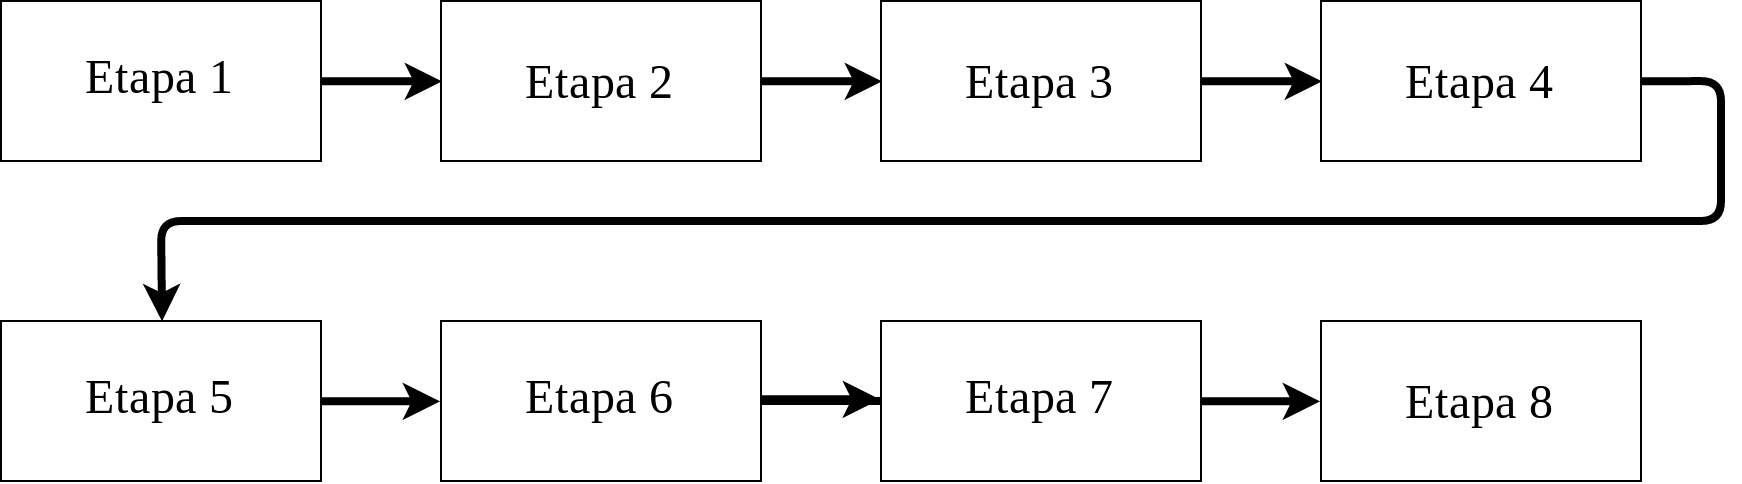
\includegraphics[width=\textwidth]{cap1_metodologia-etapas}
    \label{fig:cap1_metodologia-etapas}
    
    \footnotesize{Fonte: Elaborado pelo Autor}
\end{figure}

A seguir, a sequência de etapas demonstradas anteriormente são especificadas em detalhes.

\begin{itemize}\parskip -1pt
    \item Etapa 1: Análise e definição do escopo do trabalho.
	\item Etapa 2: Levantamento bibliográfico sobre Internet das Coisas e Sistemas de Recomendação;
	\item Etapa 3: Elaboração e desenvolvimento de um projeto de leitura e monitoramento dos produtos contidos na geladeira.
	\item Etapa 4: Implementação de um sistema de análise das interações e recomendação de produtos e receitas.
	\item Etapa 5: Desenvolvimento de um protótipo funcional que integre as Etapas 3 e 4.
	\item Etapa 6: Criação de um cenário de testes para avaliar o protótipo.
	\item Etapa 7: Avaliação e discussão dos resultados obtidos no cenário proposto.
	\item Etapa 8: Escrita do Trabalho de Conclusão de Curso.
\end{itemize}



% Colocar uma figura do fluxo
% Contextualizar para caracterizar
% O que vai usar 
% Teste
% Dizer como vai avaliar
% TODO: Descrição das etapas

\section{Organização do Trabalho} % Não é necessário, no TCC 1

Este trabalho, até o momento visando cumprir os requisitos da etapa etapa do TCC I, é divido em cinco capítulos. O \textbf{Capítulo 1} apresenta uma introdução do estado da arte das áreas envolvidas bem como a problemática do trabalho e os objetivos gerais e específicos.

O \textbf{Capítulo \ref{cap:internet_of_things}} trata da Internet das Coisas, no qual é realizada uma revisão da arquitetura para organização dos diversos componentes, das tecnologias existentes que possibilitam o desenvolvimento de novos dispositivos e, por fim, uma descrição sobre alguns dos ambientes nos quais a Internet das Coisas será incorporada nos próximos anos.

O \textbf{Capítulo \ref{cap:sistemas_de_recomendacao}} apresenta a área de Sistemas de Recomendação considerando um histórico, as principais abordagens e aplicações em que se inserem.  

O \textbf{Capítulo 4} tem por objetivo detalhar o sistema proposto apresentando uma visão lógica e uma visão física promovendo assim um entendimento do como os diversos componentes interagem e se comportam.

O \textbf{Capítulo 5} apresenta um cenário criado bem como os resultados obtidos a partir da aplicação do mesmo no sistema.

O \textbf{Capítulo 6} contém as considerações finais e os trabalhos futuros.

% O capítulo 5 é sobre a Avaliação do Sistema Proposto
% %	- Descrever um cenário
% %	- Avaliar e discutir o cenário a partir do sistema proposto
	
% O capítulo 6 é sobre Considerações Finais

% TODO: criar o arquivo para o organograma
	\chapter{Internet das Coisas}
\label{cap:internet_of_things}
%%%%%%%%   PARTE 1   %%%%%%%%
%\section{Conceito}


% TODO: INTRODUÇÃO

% Contextualização

% REVER
A tecnologia, com o passar dos anos, está cada vez mais presente nas indústrias, lares, comércios etc. ao mesmo tempo tornando-se indispensável para todas essas entidades. No entanto, nos últimos anos um novo paradigma está emergindo: a Internet das Coisas. A partir dela, a Internet vai deixar de existir como é vista hoje tornando, assim, onipresente (citar).

% O que é 

O conceito de Internet das Coisas (IoT) está relacionado à interconexão de objetos distintos através de uma rede, sendo esta, muitas vezes, a Internet. Desse modo, elementos do mundo real, que antes funcionavam de maneira independente ao meio aos quais estavam inseridos, são capazes de interagir com outros objetos à sua volta e, assim, trocar informações que possam ser relevantes permitindo a agregação de novas funcionalidades.  Além disso, a IoT abre espaço para interação 
entre o mundo físico e o digital a partir de dispositivos capazes de capturar dados físicos no meio em que estão tais como, temperatura, distância etc., representá-los digitalmente e trasmití-los para outros dispositivos.

	
O termo ``Internet das Coisas'' foi citado pela primeira vez por Kevin Ashton, diretor executivo da AutoIDCentre do MIT, em 1999 enquanto realizava uma apresentação para promover a ideia do uso de Identificadores de Radio Frequência (RFID) na etiquetagem de produtos. O uso da tecnologia beneficiaria a logística da cadeia de produção \cite{Finep2015}. Apesar de o termo IoT ter sido usado apenas em 1999, aplicações práticas da ideia já existiam anos antes. Um exemplo disso, é a torradeira que podia ser ligada e desligada via internet criada em 1990 \cite{Suresh2014}.

% TODO: Projeções de grandes companhias (número de dispositivos, expansão)

A Internet das Coisas está em grande expansão. Estima-se que em 2020 cerca de 24 bilhões de dispositivos IoT estejam conectados, implicando em cerca de quatro dispositivos por pessoa. Para tanto, em torno de 6 trilhões de dólares serão investidos em desenvolvimento de tecnologias de hardware e software, como aplicações, segurança e dispositivos de hardware. Apesar da grande quantia investida, o setor é visto como promissor. Estima-se será gerado em torno de 13 trilhões de dólares em 2025 \cite{Meola2016}

Para conectar uma grande quantidade de objetos são necessárias tecnologias, muitas delas sem fio, que permitam que os dispostivos interajam entre si trocando informações de maneira eficiente. A próxima seção tratará dessas tecnologias e a maneira com são organizadas para formar uma arquitetura. A seção seguinte apresenta alguns novos ``conceitos(sobre os smart tudo)'' que a IoT trouxe e algumas aplicações específicas para algumas das mais variadas áreas já existentes.


\section{Arquitetura}
% Escrever sobre as diversas arquiteturas existentes, características de cada uma, as melhores aplicações de cada uma etc.

% Falar sobre a inexistência de um padrão global para a IoT, mas mostrar as instituições que estão tentando tornar a IoT padronizada em realidade.

\section{Tecnologias}

% Escrever sobre as tecnologias

% ==================================================================================================
\subsection{Bluetooth}

% O que é
% MELHORAR e referenciar
O Bluetooth é uma especificação de rede WPAN, ou seja, rede sem-fio pessoal, sendo descrito e especificado pela IEEE 802.15.1. O Bluetooth foi criado na década de 90 com o objetivo de unirtecnologias distintas, tais como computadores, celulares entre outros a partir de uma padronização de comunicação sem fio entre os dispositivos \cite{Kardach2008}. 

%\begin{figure}[H]
%	\centering
%	\caption[ABC]{Interconexão entre diversas classes de dispositivos}
%	\label{key}
%	\includegraphics[width=0.7\textwidth]{img/bluetooth-ecosystem}
%    \newline Fonte: Repositório de imagens Pixabay %(link: 
%    %https://pixabay.com/en/bluetooth-connectivity-wireless-1690677/)
%\end{figure}

Uma das principais características da tecnologia \textit{wireless} é o curto alcance de transmissão variando de centímetros até alguns metros \cite{Huang2007}. 

A tecnologia vem sendo usada ao longo dos últimos anos em diversas aplicações como transferência de arquivos entre dispositivos, transmissão de áudio entre smartphones e fones sem fio, dispositivos capazes de determinar contexto, como os beacons, entre outros.

% Topologias
No IEEE 802.15.1 há suporte para criação de redes \textit{ad-hoc}, aos quais, é desnecessário uma infraestrutura de rede para conexão dos dispositivos. A partir disso é possível criar redes chamadas \textit{picorredes}, nas quais os dispositivos são organizados em até oito associados, sendo um deles um mestre, ao qual coordena as operações, e os demais escravos \cite{BluetoothSIG2017}.

% Características
A tecnologia Bluetooth opera na faixa ISM de 2.4 GHz de uso livre em modo TDM com um delta de $625\mu$s, proporcionando uma taxa de transmissão máxima em torno de 2 Mb/s, podendo variar de acordo com o dispositivo e a categoria de tecnologia de Bluetooth utilizada \cite{BluetoothSIG2017}.

% Forma de conexão.

\subsubsection{Categorias}

Segundo \citeauthor{BluetoothSIG2017}, o Bluetooth pode ser categorizado em:

\begin{enumerate}[label=(\Alph*)]
    
    \item {BR/EDR}
    %2.0 a 2.1
    
    % REVER
    Esta é a subdivisão mais popularizada do Bluetooth presente nas versões $2.0$ e $2.1$ do Bluetooth, onde as principais características são alta velocidade de transmissão alta em relação à outra categoria, baixo alcance e necessidade de conexão através de pareamento, onde os dispositivos confirmam a conexão. A partir disso, há um transmissão contínua de dados. Uma desvantagem é o consumo de energia considerável para o funcionamento do Bluetooth, já que há 
    uma conexão contínua e uma taxa de transmissão que mantêm o dispositivo ativo por um longo período ininterrupto.
    % taxa de dados
    A taxa de transmissão gira em torno de 2Mb/s.
     
    
    \item BLE
    
    % 4.0, 4.1, 4.2
    
    % O que é
    O \textit{Bluetooth Low Energy} (BLE) é a mais recente categoria do Bluetooth incorporada na versão 4.0, em 2011, além de ser a menos comum \cite{LinkLabs2015}.
    % Foco
    BLE está centrado no baixo consumo de energia para permitir que certos dispositivos não precisem recarregar ou trocar suas fontes de carga, muitas vezes uma bateria, por longos períodos, que podem chegar a anos. 
    % Pareamento
    Para uma conexão para transmissão de dados, ao contrário do BR/EPR, não é necessário um pareamento para realizá-la, além disso esta tem curta duração, na ordem de milissegundos.
    %Taxa e alcance
    Ademais, a taxa de dados é baixa e o alcance alto. A baixa taxa de dados decorre do modo de funcionamento dos dispositivos BLE, aos quais, enviam dados em rajadas, ou seja, de tempos em tempos dados são transmitidos em forma de \textit{broadcast} e os dispositivos que estiverem conectados receberão esses dados. Nos intervalos de tempo em que o dispositivo não transmite, ele ``dorme'', isto é, entra em modo de consumo mínimo a fim de poupar energia.
    
    %Aplicação
    A aplicação prática dessas características está na IoT através de \textit{beacons} e \textit{wearables}, aos quais incorporam o BLE. Os beacons foram introduzidos pela \textit{Apple} em conjunto com o iOS 7, com o nome de \textit{iBeacon}, que permitia aos aplicativos possuíssem senso de localização \cite{Apple2014}. Com esses dispositivos é possível aprimorar a experiência do usuário em estabelecimentos como museus, supermercados, shoppings, estádios, através da identificação de contexto, na qual, a partir da detecção de um beacon e da aproximação ou afastamento deste, uma aplicação móvel em um smartphone de um usuário pode exibir conteúdos, indicar promoções entre outros relacionados aquele dispositivo BLE.
    
    %\begin{figure}[H]
    %	\centering
    %	\caption[ABC]{{\noindent Alguns exemplares de beacons}}
    %	\label{fig:beacons}
    %	\includegraphics[width=0.5\textwidth]{img/beacons.jpg}
    %	\newline Fonte: Shine Solutions %(link: 
    %%https://shinesolutions.com/2014/02/17/the-beacon-experiments-low-energy-bluetooth-devices-in-action/
    %\end{figure}
    
    \item{Dual-mode}
    
    Esta categoria se refere a dispositivos, como \textit{smartphones} que precisam se conectar tanto com dispositivos BR/EDR, como fones de ouvido, e BLE, como \textit{beacons} \cite{BluetoothSIG2017a}.

\end{enumerate}


\subsubsection{Bluetooth 5.0}

A versão 5.0 do Bluetooth foi lançada em dezembro de 2016 e trás consigo aprimoramentos em desempenho e segurança, garantindo duas vezes mais velocidade, quatro vezes mais alcance, oito vezes mais taxa de dados e, por fim, maior coexistência \cite{BluetoothSIG2017b}. 

Com a nova versão, veio a flexibilidade para construção de soluções baseadas em necessidade. Parâmetros como alcance, velocidade e segurança podem ser regulados para diversos objetivos a depender das aplicações \cite{BluetoothSIG2017b}.

Algumas atualizações contribuem para a redução de interferência com outras tecnologias sem fio, dessa forma, proporciona melhor coexistência entre dispositivos Bluetooth e de outras tecnologias, dentro do cenário emergente da IoT \cite{BluetoothSIG2017b}.


% ==================================================================================================
\subsection{RFID}

O RFID (Indentificação por Rádio Frequência) é uma tecnologia de identificação automática, entre diversas outras como código de barras, cartão inteligente e procedimentos biométricos, no entanto se distingue pelo modo de funcionamento, ou seja, por ondas eletromagnéticas. Por outro lado, o RFID se destaca em relação às outras tecnologias em relação às influências externas no seu funcionamento, como sujeira, posição de leitura. Desse modo, não é necessário nem limpar ou reposicionar o dispositivo RFID para efetuar a leitura \cite{Finkenzeller2010}. 

% LEITOR E TRANSPONDER
No RFID, os dados são transmitidos através de ondas de rádio entre dois dispositivos: \textit{transponder} ou \textit{tag} e \textit{leitor}. O transponder é localizado no objeto identificado, um produto, equipamento etc., e nele são mantidos os dados de identificação. Já o leitor é responsável pela leitura e escrita dos dados presentes no transponder \cite{Finkenzeller2010}.

% FUNCIONAMENTO
Para a transmissão dos dados entre os dois dispositivos o leitor emite ondas de rádio na tag. Ao receber o estímulo, a tag responde com os dados contidos nela. Além disso, existem tags que utilizam a energia do campo eletromagnético gerado pelo leitor para seu funcionamento, sendos estas chamadas de \textit{passivas}. Existem, também, aquelas que possuem uma fonte própria de energia e por isso são denominadas \textit{ativas} \cite{Finkenzeller2010}.

Um exemplo de tag ativa é mostrada na Figura Y.

%\begin{figure}[H]
%	\centering
%	\caption[ABC]{{\noindent Exemplo tag RFID ativa}}
%	\label{fig:active-rfid}
%	\includegraphics[width=0.3\textwidth]{img/active-tag.jpg}
%	\newline Fonte: Vnsky %(link: 
%	%http://www.vnsky.com/parts/2673180/ACTIVE-TAG-REFERENCE-DESIGN-KIT.html
%\end{figure}

Uma tag passiva é mostrada na Figura Y.

%\begin{figure}[H]
%	\centering
%	\caption[ABC]{{\noindent Exemplo tag RFID passiva}}
%	\label{fig:passive-rfid}
%	\includegraphics[width=0.3\textwidth]{img/passive.png}
%	\newline Fonte: Eletrosome %(link: 
%	%https://electrosome.com/rfid-radio-frequency-identification/
%\end{figure}

% TIPOS (alimentação)

% ATIVO
% PASSIVO

% FREQ. DE OPERAÇÃO
Uma das características mais importantes dos dispositivos RFID é a frequência de operação já que ela influi no distância máxima de operação. Tal fator é determinado pelo leitor. Os dispositivos são classificados, de acordo com a frequência de operação, em três grupos:

\begin{itemize} \parskip -4pt
	\item \textbf{LF (Baixa Frequência):} Entre 30kHz à 300kHz
	\item \textbf{HF (Alta Frequência):} Entre 3MHz à 30MHz
	\item \textbf{UHF (Ultra Alta Frequência)}: Entre 300MHz a 3GHz.
\end{itemize}

É possível distinguir pelo alcance:

\begin{itemize} \parskip -4pt
	\item \textbf{\textit{Long-range} ou longo alcance:} maior que um metro.
	\item \textbf{\textit{Remote-coupling} ou ligação remota:} até um metro
	\item \textbf{\textit{Close-coupling} ou ligação próxima:} até um centímetro.
\end{itemize}

%TODO: Escrever sobre os fatores que influenciam no funcionamento, alcance etc.

% ==================================================================================================
\subsection{NFC}
% O_QUE É
O NFC é um sistema de comunicação sem fio derivado do RFID. Ele permite transações simples e seguras entre dois dispositivos a partir da curta distância de operação, em torno de 4cm, e do funcionamento baseado em aproximação dos objetos em questão \cite{NFCForum2016}. 
Assim, é possível realizar leituras de tags e obter conteúdos de acordo com a aplicação, transferir dados entre smartphones entre outras funcionalidades.

% COMPATIBILIDADE
Outra vantagem do NFC é a compatibilidade com a infraestrutura de cartões sem contato existentes permitindo usar um único dispositivo em tecnologias diferentes. Desse modo, é possível interagir com tags RFID, por exemplo.


% FUNCIONAMENTO
Como o RFID, o NFC funciona através de ondas eletromagnéticas com uma taxa de transmissão máxima de 424kbps \cite{NFCForum2016}. Além disso, pode operar em dois modos de comunicação \cite{Igoe2014}: ativo e passivo. Assim como no RFID, é possível que os dispositivos NFC que contenham os dados usem a energia do leitor para transmitir seus dados, no modo passivo, ou usem uma fonte própria para tal procedimento, no modo ativo.


% MODOS DE OPERAÇÃO
Outra característica importante no NFC são os modos de operação. De acordo com \citeauthor{NFCForum2016} existem três modos:

\begin{itemize} \parskip -4pt
	\item \textit{Leitor/Escritor de tag}: Tem por objetivo ligar o mundo físico ao digital através 
	de aplicações que leem e/ou escrevem em tags para obter dados e, assim, fornecer conteúdo ao 
	usuário relacionado à tag lida. Um exemplo é um smartphone ao ler uma tag NFC de um cartaz na 
	rua.
	\item \textit{Peer to Peer}: Visa conectar dispositivos por aproximação física e permite troca 
	de arquivos. Um exemplo é o Android Beam que permite troca de arquivos entre smartphones com o 
	sistema operacional da Google.
	\item \textit{Emulação de cartão}: Conecta o dispositivo do usuário em uma infraestrutura 
	possibilitando a simulação de um cartão, além da realização de transações financeiras e 
	identificação no sistema de transporte a partir da aproximação do dispositivo a um leitor 
	específico.
\end{itemize}

% CATEGORIAS
Há quatros tipos de tags definidas \cite{NFCForum2016a}, sendo que todos operam no modo Leitor/Escritor descrito anteriorente : 

\begin{itemize} \parskip -4pt
	\item \textbf{Tipo 1}: 96 bytes de memória disponível e expansível para 2kiB. Usuário pode 
	configurá-la para somente leitura.
	\item \textbf{Tipo 2}: 48 bytes de memória disponível e expansível para 2kiB. Usuário pode 
	configurá-la para somente leitura.
	\item \textbf{Tipo 3}: Baseado no padrão industrial japonês e conhecido como FeliCa. Pode ser 
	configuradas para leitura/escrita ou somente leitura na fabricação. A memória disponível varia, 
	mas com um limite teórico de 1MiB por serviço.
	\item \textbf{Tipo 4}: A memória disponível varia estando acima de 35 kiB por serviço. É 
	possível ser configurada para leitura/escrita ou somente leitura.
\end{itemize}

O NFC possui um padrão com o qual dispositivos devem estar formatados, o NDEF (\textit{NFC Data Exchange Format}) um formato comum de comunicação \cite{Igoe2014}. Desse 
modo, os dados armazenados em tags devem estar gravados nesse formato. A partir do NDEF é possível armazenar e trocar documentos binários como MIME, que incluem imagens, arquivos PDF entre outros, 
URL, texto simples entre outros.


% ==================================================================================================
\subsection{Zigbee}

% WHAT IS IT
O Zigbee é um protocolo padrão de comunicação de baixa-potência para redes sem-fio \textit{mesh}, ao qual permite a diversos dispositivo trabalharem em conjunto \cite{Faludi2011}.

O Zigbee é descrito como um conjunto de camadas implementadas sobre o IEEE 802.15.4 \cite{Faludi2011}, ao qual especifica a camada física(PHY) e o controle de acesso ao meio (MAC) para redes sem-fio de baixa potência \cite{IEEE2011}.

As camadas do Zigbee, de acordo com \cite{Faludi2011}, fazem:

\begin{itemize} \parskip -4pt
	\item \underline{Roteamento:} Tabelas de roteamento que definem como um nó envia dados até um 
	destino
	\item \underline{Rede Adhoc:} Criação automática de rede
	\item \underline{\textit{Self healing mesh}:} Descobe se nós se perderam da rede e a 
	reconfigura para garantir uma rota para os dispositivos conectados ao nó faltantes
\end{itemize}

O Zigbee opera na faixa não licenciada ISM, de 2,4GHz, o que permite sua expansão global e, assim, ser capaz de operar em qualquer local do mundo.

O Zigbee especifica que os nós das redes criadas possam assumir papeis específicos. Cada nó deve 
assumir uma das categorias a seguir \cite{Faludi2011}:

\begin{itemize} \parskip -4pt
	\item \textit{Coordenador}: Responsável por criar a rede, distribuir endereços, manter a rede segura, 
	mantê-la em funcionamento entre outras funções que caracterizam a rede. Cada rede tem um e 
	apenas um coordenador.
	\item \textit{Roteador}: Tem capacidade de unir redes existentes, enviar e receber informações e rotear 
	informações, atuando como um intermediário entre dispositivos que, por estarem muito distantes 
	entre si, não podem se comunicar diretamente. É permitido às redes terem múltiplos roteadores, 
	podendo também não possuírem nenhum e, caso exista, cada roteador deve estar conectado a um 
	coordenador ou outro roteador.
	\item \textit{Dispositivo final}: É um tipo de nó capaz de se unir a redes além de enviar e receber 
	informações da rede. Além disso, podem se desligar de tempos em tempos para poupar energia. 
	Caso mensagens para um dispositivo final desligado sejam detectadas, o nó responsável por ele, 
	podendo ser um coordenador ou roteador, armazena as mensagens até que o nó desperte.
\end{itemize}

Há diversas topologias suportadas, nas quais, englobam os três tipos de nós e suas possíveis 
maneiras de organização \cite{Faludi2011}:

\begin{itemize} \parskip -4pt
	\item \textit{Par a par}: Uma rede formada apenas por dois nós, sendo um deles, obrigatoriamente, um 
	coordenador e nó restante podendo ser um roteador ou dispositivo final.
	\item \textit{Estrela}: Nessa topologia, o coordenador se situa no centro da rede e os demais nós, 
	roteadores ou dispositivos finais, conectados apenas a ele, formando uma rede no formato de 
	estrela.
	\item \textit{Mesh}: Os dispositivos finais circundam os demais nós roteadores e coordenador. O 
	coordenador e roteadores atuam como intermediários, roteando mensagens para dispositivos 
	finais, outros roteadores ou para o coordenador. Apesar da nova função do coordenador, este 
	permanece no controle e gerenciamento da rede.
	\item \textit{Cluster tree}: Nessa topologia, cada roteador é responsável por um conjunto de 
	dispositivos finais. As mensagens vindas desses dispositivos devem ser encaminhadas 
	primeiramente para seu roteador responsável para então ser encaminhada ao destino na rede.
\end{itemize}

% TODO: Colocar ilustração das topologias

O Zigbee define três maneiras de identificação de nodos, que podem utilizadas em uma aplicação para 
diferenciar os nós.

\begin{itemize} \parskip -4pt
	\item 64 bits: Único e permanente para cada rádio fabricado.
	\item 16 bits: Dinamicamente configurado pelo coordenador ao entrar em uma rede. É único apenas 
	dentro do contexto da rede.
	\item Node Id: Pequena cadeia de texto. Não é possível garantir sua unicidade em nenhum 
	contexto, apesar disso, é mais amigável aos olhos humanos.
\end{itemize}

%\subsubsection{Criação de uma rede}

%Cada rede de sensores deve possuir um identificador chamado endereço PAN (Personal Area Network). 
%Além disso, cada nó deve ter o mesmo PAN configurado e o mesmo canal de comunicação, que é escolhido de acordo com a disponibilidade pelo coordenador. 

%Para que uma mensagem chegue a um destino, é necessário que o nó emissor tenha conhecimento do endereço do nó destinatário do pacote.

%\subsubsection{XBee}

%O XBee é um dispositivo fabricado pela Digi. Existem cerca de 
%30 combinações de hardware, protocolos de \textit{firmware}, potência de transmissão e antenas.

%Apesar das diversas combinações, há duas versões básicas do XBee: Série 1 e Série 2.

%Os nós XBee Série 1 proveem comunicações ponto a ponto, bem como uma implementação proprietária de 
%rede \textit{mesh}. Já os nós Série 2 permitem diversas derivações de padrões de redes mesh Zigbee.

% IMAGEM XBEE S1 e XBEE S2
% ==================================================================================================

\subsection{Wifi}
% O que é
% Features
% História
% Categorias
% Oportunidades


\subsection{Outros}
% Z-wave
Entre as tecnologias utilizadas em Smart Homes está o Z-Wave, um protocolo sem fio focado em automação residencial e comercial de pequeno porte, criado pelo ZenSys e hoje representado pela Z-Wave Alliance  (whan survey, gomez, 2010). O protocolo foi desenvolvido especificamente para controle, monitoramento e verificação de estado. Em relação a aspectos técnicos, o Z-Wave opera na faixa de frequências de 1GHz, o que evita interferências com outras tecnologias como Bluetooth e Wifi que operam em 2,4GHz. Entre as principais vantagens do Z-wave está a interoperabilidade que este proporciona entre os diversos produtos desenvolvidos com a tecnologia, além da segurança obtida a partir do uso de criptografia AES128.  (http://z-wavealliance.org/about_z-wave_technology/)

% 6LowPan
Há a tendência de dispositivos IoT conectados à Internet usaram o protocolo de endereçamento IPv6 para serem identificados na rede. No entanto, algumas das aplicações terão limitações como fonte de energia e capacidade de transferências de dados limitadas. A partir disso, criou-se o 6LowPan, focado em dispositivos com restrições de consumo de energia. A principal característica desse protocolo é a redução da transmissão de dados a partir da compressão dos cabeçalhos do IPv6. Com isso, o 6LowPan é capaz de reduzir a sobrecarga de pacote para dois bytes. (enabling technologies)
(rever com base em http://www.ti.com/lsds/ti/wireless-connectivity/6lowpan/overview.page)

\section{Ambientes inteligentes}

\subsection{Smart grid}

\textit{Smart grid} é uma rede elétrica inteligente, na qual, através da tecnologia coleta dados de consumo e dos distribuidores toma ações a partir deles, tornando o sistema mais eficiente, seguro e sustentável \cite{Cecilia2016}. As smart grids têm três componentes importantes: rede de transmissão inteligente, às quais contêm sensores, troca de informações, controle e tecnologias de comunicação que proporcionam uma transmissão eficiente, tecnologia da informação e comunicação de smart grid  e tecnologia de medição inteligente, no qual, além de realizar medições como os equipamentos tradicionais, é capaz de trocar informações com a rede inteligente. 

Empresas como a \textit{Texas Instruments} (TI) têm investido em soluções para smart grid que proporcionam segurança, eficiência e inteligência. A TI oferece soluções para monitoramento da rede através de medidores de eletricidade, gás e calor, além de tecnologias para comunicação como o 
\textit{Power Line Communications} entre outras \cite{TexasInstruments2017}.

\subsection{Smart home}

% TODO: Conceitos
O conceito de \textit{smart home} ou casa inteligente propõe um novo modelo para um ambiente domiciliar no qual a implementação e o uso da tecnologia abrem espaço para novas formas de interação com o lar, além de proporcionar mais comodidade e um melhor gerenciamento dos equipamentos presentes. Isso será possível graças ao uso de sensores e atuadores no ambiente, nos eletrodomésticos e utensílios. Além disso, para interconectar todos os dispositivos, usa-se as tecnologias de rede existentes, como o Zigbee e a Internet.

A interconexão dos dispositivos em uma casa inteligente proporcionorá funcionalidades inéditas de interação de acordo com as ações do morador, como entrar e sair de um cômodo da casa. Nesse caso, seria possível implementar um sistema que apagasse e acendesse a lâmpada conforme os sensores de presença indicarem a ausência do indivíduo e a hora do dia \cite{audiovideo}.

Entre as principais apostas para as casas inteligentes está o aumento da eficiência do consumo energético. O uso da tecnologia por meio de medidores de energia, tomadas e aparelhos inteligentes permitirá o monitoramento e controle do consumo dos dispositivos da casa. Com base nisso, é viável a otimização do consumo de cada equipamento controlando-o para ativá-lo somente quando necessário e, assim, evitar desperdícios, além de previsão da demanda de energia para cada momento do dia (A review, Stojk).

% Segundo \cite{DeSilva2012}, as casas inteligentes podem ser divididas em três categorias principais. 
% A primeira delas atenta-se em detectar e reconhecer ações dos moradores e seu estado de saúde e, baseando-se nelas, prover serviços com foco no bem-estar e na saúde dos residentes. Nesse categoria estão incluídos cuidado de idosos, da saúde e de crianças. 
% A segunda categoria se refere à captura e multimídia de eventos ocorridos no dia a dia.
% A terceira tem como foco na segurança. Uma sistema de alerta pode ser ativado, no momento em que uma invasão, sequestro ou desastre natural ocorrer, a partir captura de imagens, sensoriamento entre outros.



XXXXXXXXXXXXXXXXXXXXXXXXXXXXXXXXXXXX

% TODO: Arquitetura
    % Categorias

As casas inteligentes necessitam que os dispositivos sejam organizados hierarquicamente para garantir um bom desempenho. \citeauthor{stojkoska} propõe uma arquitetura para casa inteligente construída a partir de alguns componentes:  \textit{smart objects}, hubs, cloud e aplicações de terceiros (escanoladores, reguladores, balanceadores de carga).
(stoj...; mostrar a figura do cara)

 Os objetos inteligentes interagem diretamente com o ambiente e com os moradores, seja de forma direta, no caso de eletrodomésticos inteligentes ou ubíqua no caso de sensores.

 A partir da incorporação da tecnologias aos objetos da casa será possível obter informações inétidas sobre estes e sobre os moradores, como temperatura ambiente preferencial, grau de uso dos equipamentos entre outros.
 Muitos serviços poderão ser automatizados. Acender e apagar de luzes, ativação do condicionamento de ar, cafeteira etc. \cite{Silva2012}.


% TODO: Formas de interação
    % Vídeo
    % Áudio
 A partir da interação diária dos moradores com os eletrodomésticos e móveis da casa e do uso de recursos de imagem, áudio e vídeo, será possível capturar ações e eventos do dia a dia, como o entrar e sair de um quarto por exemplo. Com base nisso, será possível adaptar os equipamentos da casa para que automaticamente executem ações para cada evento do dia a dia {stoj...}.

Uma casa inteligente permite que os moradores tenham maior independência no seu dia a dia, especialmente em caso de pessoas idosas, com dificuldade de locomoção, além daquelas com deficiências físicas e visuais.
No artigo X, os autores propõe um sistema que usa imagem para casa inteligente, capaz de detectar o dia a dia de uma pessoa idosa. É possível também identificar possíveis quedas e avisar o responsável ou ao atendimento médico.

% Rascunho
Entender o comportamento dos moradores a partir da detecção de suas ações é desejável para que se possa prover serviços que vão de acordo com o esperado por eles.

% TODO: Usuários

Despite this broad range of potential and assumed benefits, a clear user-centric vision of smart homes is currently missing from a field being overwhelmingly ‘‘pushed’’ by technology developers ( smart home and their users).

% TODO: Tecnologias
    % Tecnologias de 
    % Eclipse SmartHome

Diversas sistemas para vem sendo implementados nos últimos tempos para facilitar o desenvolvimento de aplicações e dispositivos para casas inteligentes.
Entre eles está o projeto SmartHome do Eclipse para IoT.
(imagem do projeto)
    
% TODO: Desafios

A empresa \textit{Amazon}, empresa de tecnologia dos Estados Unidos, oferece o \textit{Amazon Echo}, um dispositivo que oferece diversas funcionalidades multimídia, como reprodução de músicas através de controle por voz, inclusive se algo estiver tocando, além de oferecer informações como previsão 
do tempo, notícias, tráfego entre outros através do \textit{Alexa Voice Service}. É capaz de controlar a luz, tomadas e termostatos além de ser compatível com produtos de empresas, como Samsung, Philips entre outras, com foco em \textit{smart homes} \cite{amazon2017}.

\subsubsection{Smart Kitchen}

Seguindo a lógica das casas inteligentes, as \textit{Smart Kitchens} ou cozinhas inteligentes promovem o aprimoramento dos dispositivos da cozinha com a inserção da tecnologia. A partir disso, utensílios como panelas, talheres entre outros poderão fazer uso de tecnologia para entregar novas funcionalidades. Por exemplo, no caso das panelas, é possível colocar sensores de temperatura e câmera para determinar a temperatura atual e o estado atual do alimento que está sendo cozido. A partir disso, o sistema computacional presente na panela, processará os dados e fará uma comunicação com o fogão para ajustar a intensidade do fogo caso ainda não esteja pronto, ou simplesmente, desligar o fogo, caso o esteja. 

\subsection{Smart factory}
% Quarta revolução industrial,

% Apoio a logística

%\subsection{Transportes}


%A empresa \textit{General Eletric} (GE), a maior empresa digital industrial do mundo, atua em diversos setores como saúde, aviação, transporte, energias renovável, entre outros \cite{generalelectric2017} . A empresa fabrica uma locomotiva, modelo \textit{Evolution}, com cerca de 250 sensores, resultando em 150 mil leituras por minuto. Com a leitura dos sensores, dados como tempo, pressão de óleo, temperatura, velocidade entre outros, podem ser utilizado para determinar a performance da máquina em um dado momento. Além disso, é possível prever quando surgirá algum problema, devido a algum componente que indica falha, a partir do software de análise em escala industrial \textit{Predix} \cite{danielterdiman2014}.

\subsection{Smart City}

\subsection{Wearables}

\textit{Wearables} são dispositivos computacionais vestíveis, ou seja, são itens que uma pessoa pode usar no dia a dia como, roupas, relógios, óculos, sapatos entre outros e, ainda obter novas funcionalidades, graças à presença da tecnologia nesses dispositivos. Isso é possível devido a sensores aos quais medem sinais vitais do corpo humano e dados do ambiente, a depender da aplicação, além de pequenos equipamentos de hardware responsáveis por ler os dados dos sensores e comandos do usuário e assim tomar as ações necessárias de acordo com a situação.

Os \textit{wearables} têm aplicações nas mais diversas áreas, partindo das áreas da saúde e esportes até lazer e trabalho. 

Algumas empresas têm investido na área de dispositivos vestíveis. Um exemplo é a Microsoft que vem desenvolvendo o \textit{Holo Lens}, um dispositivo que se assemelha a um óculos, com foco em realidade aumentada. A tecnologia pode ser usada na concepção e design de produtos, educação, astronomia entre outros.

Outra tecnologia em ascensão é o \textit{smart watch}, relógio digital conectado à internet, dotado de aplicativos entre outras funções que vão além de mostrar as horas.

Na área de esportes e saúde, existem as \textit{smart bands}, pulseiras capazes de monitorar sinais, como batimentos além das calorias eliminadas durante um exercício, distância percorrida entre outros.





%\subsection{Turismo}
% Exemplo de turismo do artigo
%Uma aplicação proposta consiste em um sistema de informação turístico com intuito de expandir a experiência dos visitantes nos diversos pontos turísticos no Japão. Isso é possível graças ao uso de beacons, sensores sem fio descritos na seção anterior, e realidade aumentada, viabilizada por uma aplicação móvel \cite{SHIBATA2016}. 


\section{Desafios}


\subsection{Interoperabilidade}


\subsection{Segurança}
	\chapter{Sistemas de recomendação}
\label{cap:sistemas_de_recomendacao}

\section{Histórico}


\section{Aplicações}
%	\chapter{Sistema proposto}
\label{cap:sistema_proposto}
%	\chapter{Aplicação do Modelo e Análise dos Resultados}
\label{cap:avaliacao_sistema}

Nesse capítulo será realizada a apresentação dos resultados obtidos a partir da aplicação do modelo proposto materializado em um sistema computacional a um cenário de estudo.

%%%%%%%%%%%%%%%%%%%%%%%%%%%%%%%%%%%%%%%%%%%%%%%%%%%%%%%%%%%%%%%%%%%%%%%%%
\section{Introdução}

As discussões nesse capítulo estão decompostas em três partes, sendo elas:

\begin{itemize}[noitemsep,topsep=5pt]
    \item \textbf{Fluxo de execução do sistema:} Apresenta a dinâmica do sistema a começar pela leitura dos produtos contidos na geladeira e finalizando na apresentação de recomendações e receitas, além de algumas funcionalidades, dentre as descritas no Capítulo 4.
    \item \textbf{Cenário de Aplicação:} Apresenta o cenário em que o sistema será avaliado. Assim, detalha-se o ambiente da simulação, os dados utilizados, sua obtenção, organização, além das ações executadas pelo sistema.
    \item \textbf{Avaliação do Protótipo:} Nesta seção, a partir do cenário proposto, serão demonstradas as interações com o protótipo e o resultado das interações, seja na forma de recomendações de produtos e receitas ou através de informações de estado da geladeira e de produtos contidos nesta.
\end{itemize}

%%%%%%%%%%%%%%%%%%%%%%%%%%%%%%%%%%%%%%%%%%%%%%%%%%%%%%%%%%%%%%%%%%%%%%%%%
\section{Fluxos de Execução do Sistema} \label{sec:fluxos-de-execucao}

No sistema diversas operações são executadas, às quais incluem os diversos componentes que o compõem. A seguir, são apresentados e explanados alguns fluxos de execução.

% Demonstrar fluxo de execução da leitura de conteúdo
\subsection{Leitura de Conteúdo}

No momento em que a geladeira for ligada, conforme a Figura \ref{fig:cap5_diagr_leitura}, o sistema será inicializado e as portas (ou terminais) serão configurados a fim de permitir a comunicação com os leitores e com o mecanismo de fechamento. Ademais, os eventos, disparados pela mudança do estado da porta, também são configurados. Após a conclusão das ações mencionadas, o sistema entra em modo de espera.

A partir desse ponto, o sistema dependerá da ação do usuário para operar. Assim, quando o usuário abrir ou fechar a porta, o sensor de fechamento irá propagar um novo sinal para o sistema. Quando o evento de mudança ocorre verifica-se qual o tipo de evento ocorreu, ou seja, abertura ou fechamento. Caso aberto, o sistema entra em modo de espera por alguns segundos até prosseguir com a operação, garantindo que a porta esteja realmente aberta e reduzindo as chances de ruídos interferirem no funcionamento do leitor. Além disso, garante-se que o usuário tenha tempo suficiente para fechar a porta de maneira voluntária. 

Após o período transcorrer, uma nova leitura é realizada e caso ainda aberta, um registro de porta aberta é enviado ao servidor. Caso for verificado, após a interação do usuário, que a porta está fechada, espera-se também alguns segundos. Após esse tempo, um comando de leitura é enviado para os leitores de etiquetas. Estes, por sua vez, realizam a captura das informações das \textit{tags} ao alcance e as enviam ao sistema da geladeira. Por fim, um registro de interação é enviado no servidor e gravado na base de interações.

\begin{figure}[H]
    \caption{Fluxo de leitura do conteúdo da geladeira}
    \label{fig:cap5_diagr_leitura}
    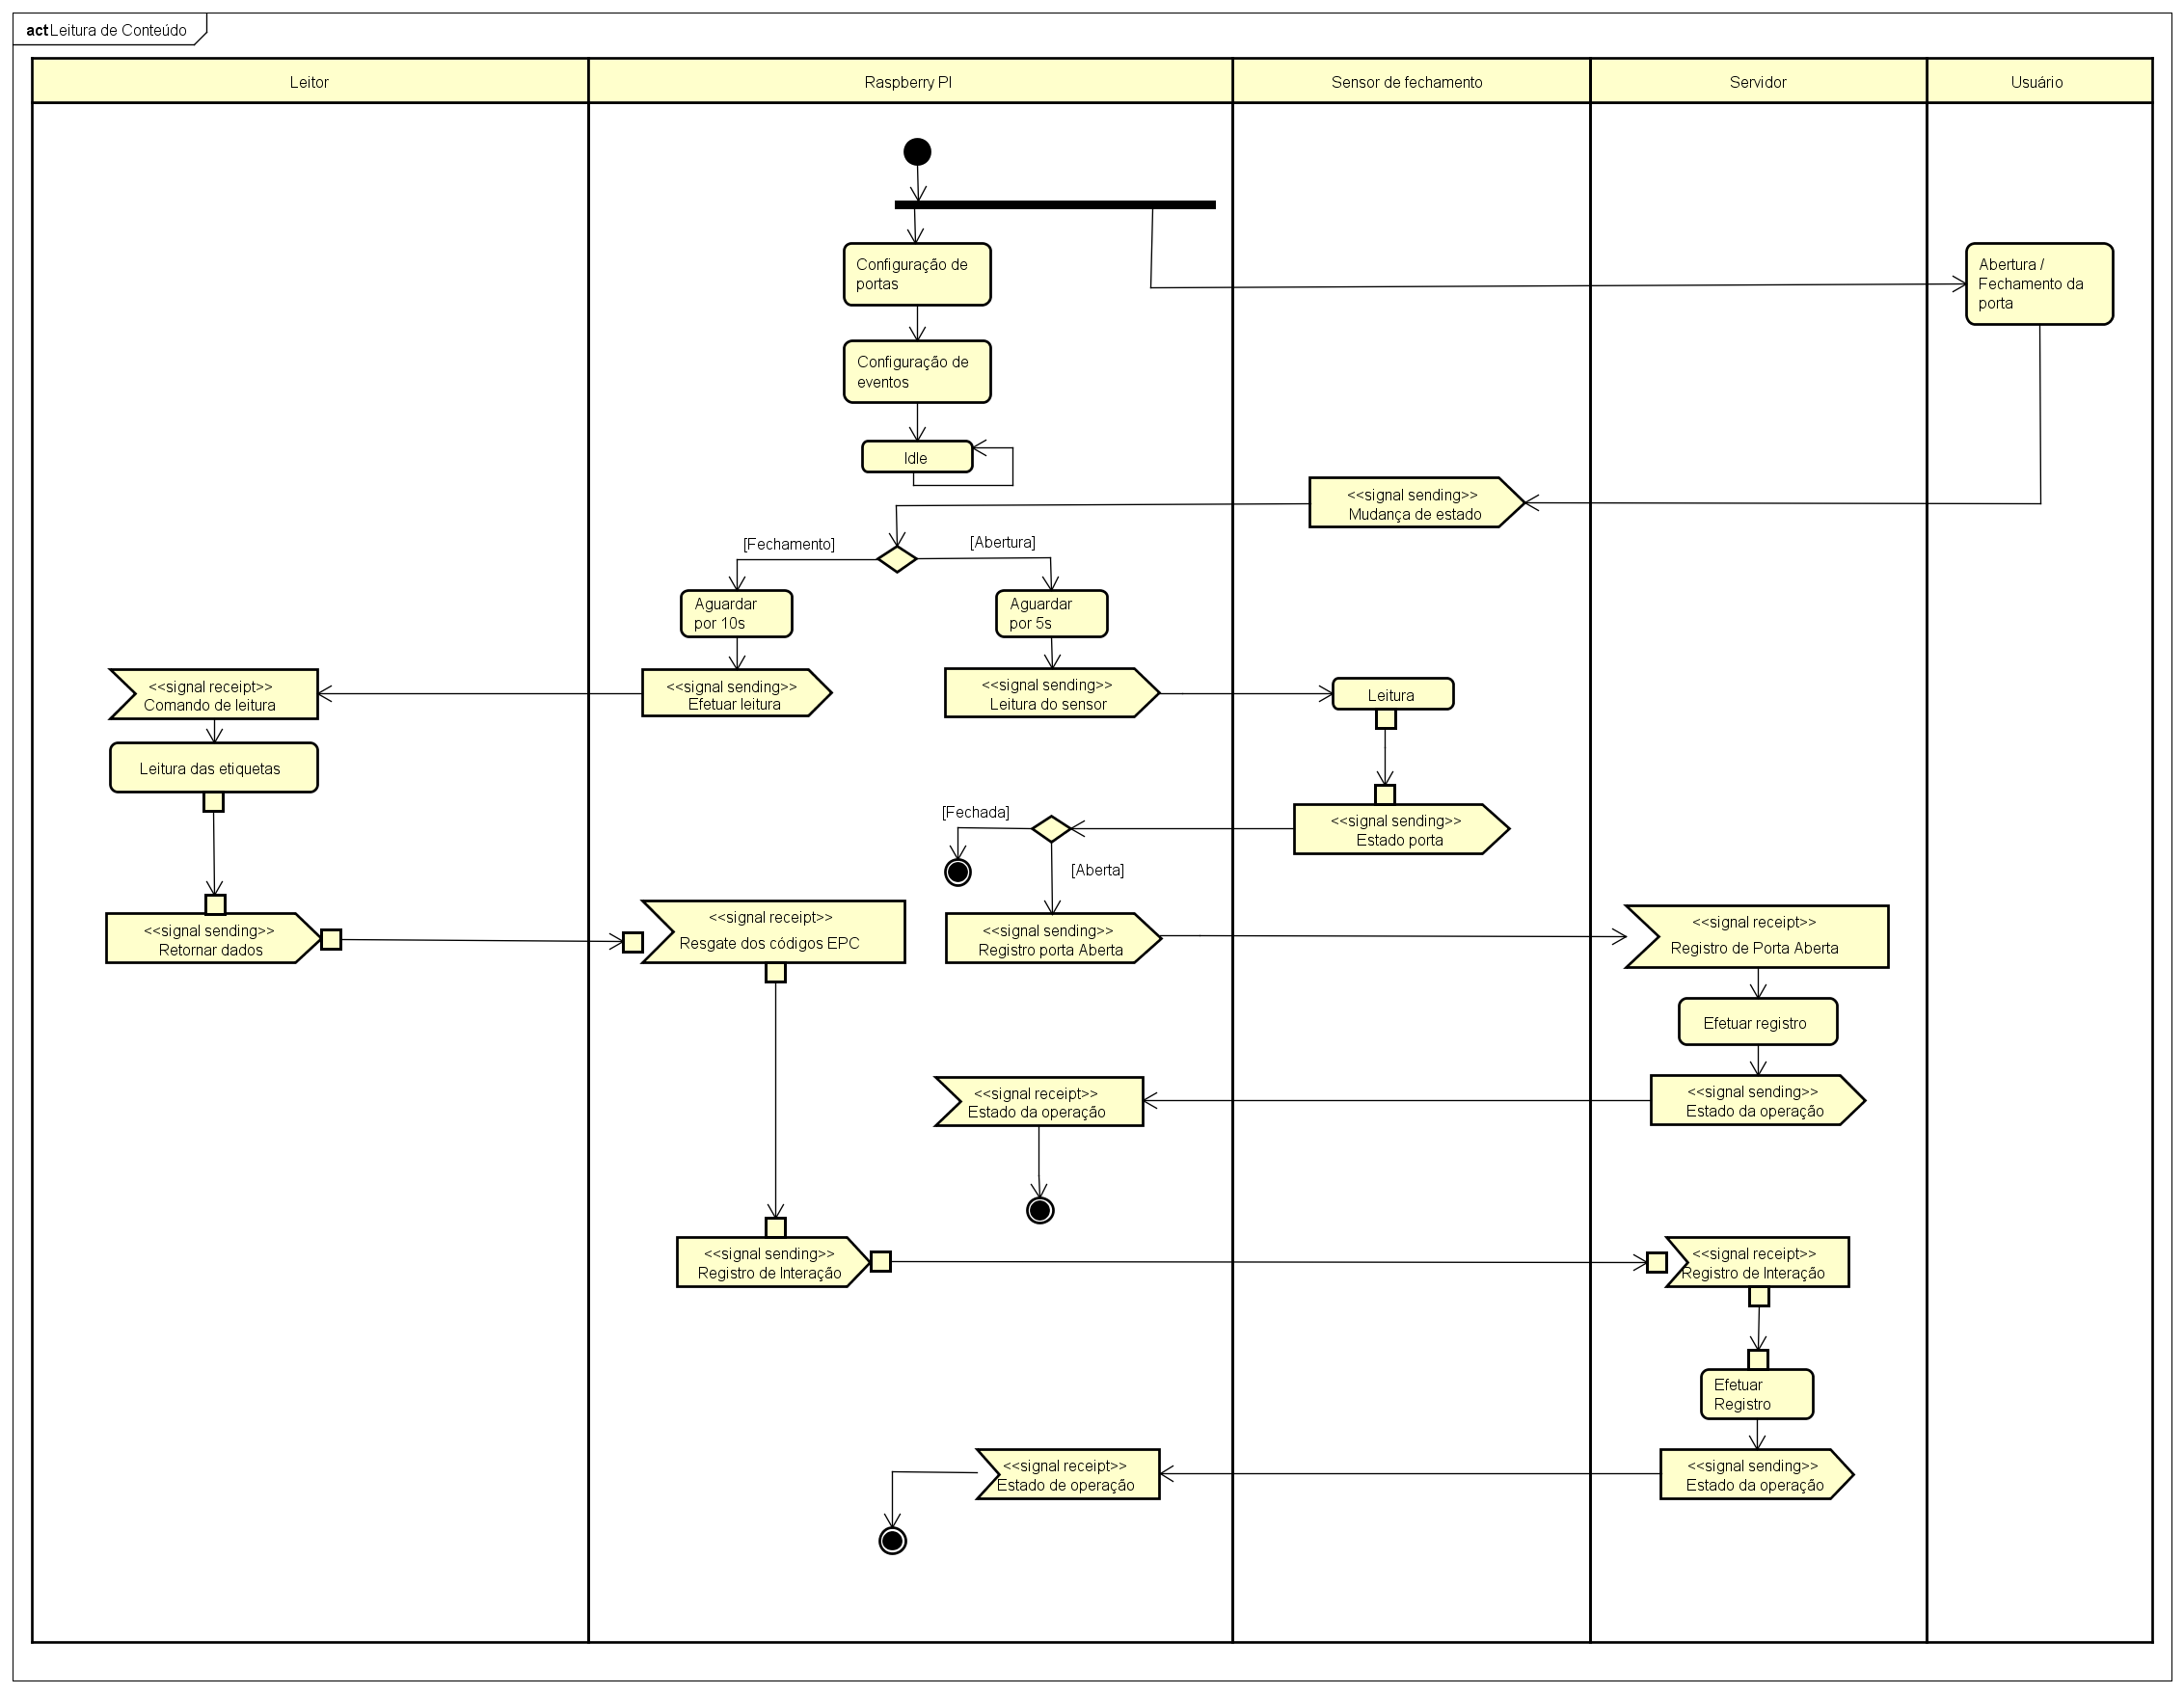
\includegraphics[height=0.9\textwidth, angle=90]{diagramas/diagr_leitura.png}
    
    \footnotesize{Fonte: Elaborado pelo Autor}
\end{figure}

%%%%%%%%%%%%%%%%%%%%%%%%%%%%%%%%%%%%%%%%%%%%%%%%%%%%%%%%%%%%%%%%%%%%%%%%%
\subsection{Listagem do Conteúdo da Geladeira}

Como  continuação do processo anterior, o processo de listagem de produtos disponibiliza na interface de usuário o conjunto de produtos disponíveis. A Figura \ref{fig:cap5_diagr_lista_prod} demonstra o fluxo de atividades para este processo.

O gatilho para tal ação é provido na interface de usuário e esta enviará uma requisição da lista de produtos referentes à uma geladeira específica. Ao receber a solicitação, o servidor realiza uma busca na base de interações pelo último registro gravado ao qual contém os códigos EPC lidos das etiquetas. Após isso, tendo o conjunto de códigos EPC, fará uma busca pelo produto correspondente a cada um. Assim, se terá uma lista de produtos e suas respectivas quantidades. Por fim, a lista de produtos, em formato JSON, é retornada à interface e apresentada ao usuário.

% Demonstrar fluxo de execução de listagem de produtos
\begin{figure}[htb]
    \caption{Fluxo para listagem de conteúdo da geladeira}
    \label{fig:cap5_diagr_lista_prod}
    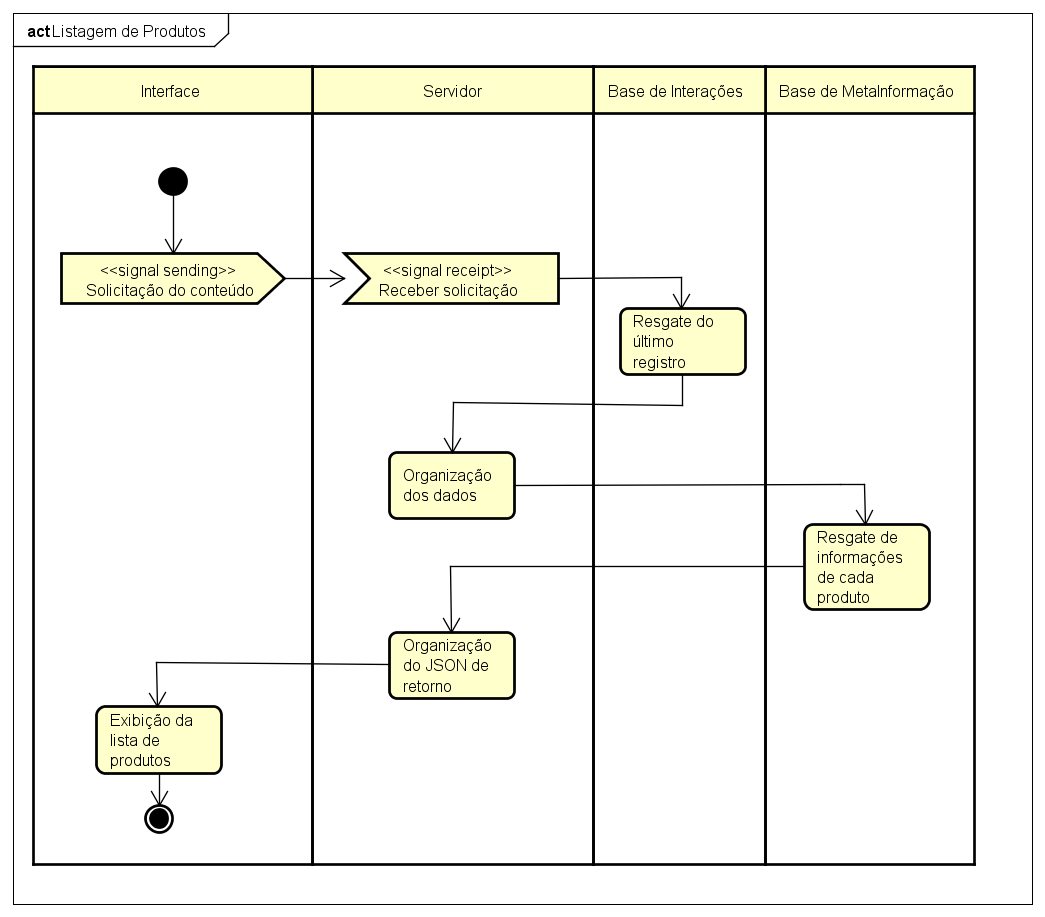
\includegraphics[width=\textwidth]{diagramas/diagr_lista_prod.png}
    
    \footnotesize{Fonte: Elaborado pelo Autor}
\end{figure}

\subsection{Recomendação de Produtos Novos} \label{ssec:geracao_rec_novo}

O processo de geração de recomendações, como já dito, é automaticamente inicializado pelo servidor, conforme Figura \ref{fig:cap5_diagr_geracao_rec}. Inicialmente, a matriz de frequência de interações de usuários com produtos é criada. Vale destacar, que um usuário está relacionado à uma geladeira. Em seguida, busca-se na base de interações todas as interações armazenadas. A partir das interações, na base de metainformação é efetuada a combinação entre códigos EPC e código de barras. A matriz de frequências é, então, preenchida com os dados obtidos no processo anterior.

Como parte do cálculo da correlação de Pearson, a média de interações de cada usuário deve ser calculada. Logo após, é computada a similaridade com a Equação \ref{eq:correlacao-pearson} entre os pares de usuários, indicados na Figura \ref{fig:cap5_diagr_geracao_rec} como $U1$ e $U2$.

Utilizando as similaridades calculadas inicia-se o processo de recomendação para cada usuário ($U1$) cadastrado no sistema. Inicialmente, o conjunto de similaridades do usuário $U1$ com os demais é ordenado em ordem decrescente, ou seja, do usuário com maior similaridade ao menor. Em seguida, para cada usuário $U2$ na lista de similaridades é realizada uma subtração de conjuntos de produtos aos quais $U2$ interagiu pelos itens que $U1$ interagiu. Assim, tem-se um conjunto de produtos que $U1$ não conhece e que poderão ser sugeridos como novas opções de compra. 

O processo citado é repetido até que todos os indivíduos na lista de usuários similares forneçam recomendações ou quando o número máximo de produtos recomendados for atingido. E quando uma das duas possibilidades ocorrer, o conjunto de recomendações será salvo na base de recomendações e o processo de recomendação se repetirá para o próximo usuário.

% Demonstrar fluxo de execução de geração de recomendação
\begin{figure}[H]
    \caption{Fluxo para recomendação de produtos novos} 
    \label{fig:cap5_diagr_geracao_rec}
    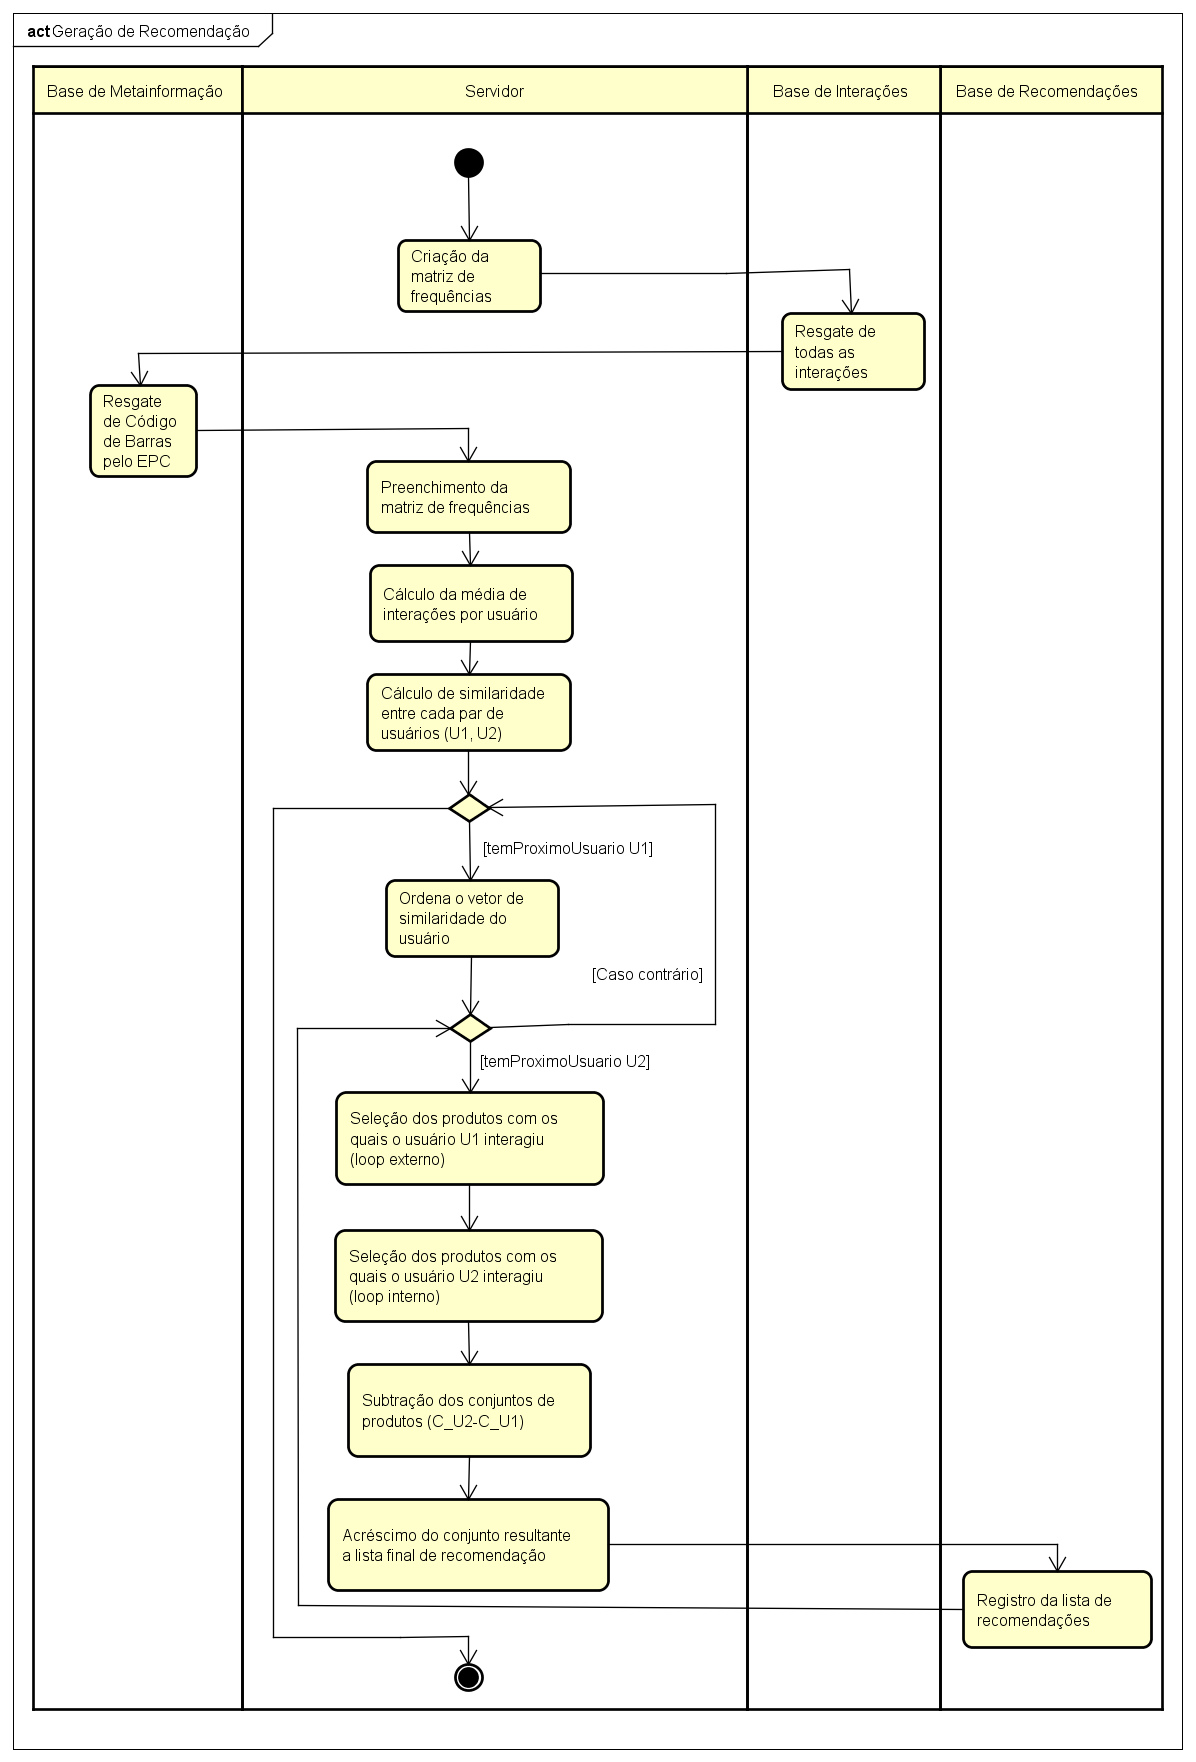
\includegraphics[width=\textwidth]{diagramas/diagr_geracao_rec.png}
    
    \footnotesize{Fonte: Elaborado pelo Autor}
\end{figure}

%%%%%%%%%%%%%%%%%%%%%%%%%%%%%%%%%%%%%%%%%%%%%%%%%%%%%%%%%%%%%%%%%%%%%%%%%
\subsection{Recomendação de Produtos Faltantes} \label{ssec:cap5_rec_prod_falt}

Da mesma forma que a seção anterior, o processo de recomendação é iniciado automaticamente pelo servidor, conforme Figura \ref{fig:cap5_rec_produto_faltante}. A partir disso, para que se recomende produtos é necessário ter as listas de produtos disponíveis atualmente e de produtos requisitados. Para tanto, inicialmente, a base de interações é consultada para o resgate da última interação, tendo esta a indicação dos itens mais recentes. A partir da lista de códigos EPC extraídos das interações é realizada uma consulta à base de metainformação para que sejam obtidos os dados dos produtos.

O próximo passo consiste na obtenção, na base de estruturas auxiliares, das informações de configuração do usuário, às quais indicam os produtos essenciais. A partir da extração dessas informações é efetuada uma comparação de quantidade entre produtos disponíveis e essenciais. Caso o produto essencial esteja disponível na quantidade necessária, nada acontece. No entanto, caso o produto esteja disponível e em quantidade insuficiente, este é inserido na lista de recomendações tendo como quantidade sugerida a diferença entre o valor necessário e o existente. Caso o produto necessário não exista, sugere-se a quantidade total indicada nas configurações.

A seguir, para o conjunto de produtos recomendados, é executada uma verificação no mercado sobre a disponibilidade dos mesmos conforme a quantidade especificada no passo anterior. Assim, caso o item esteja acessível, uma indicação positiva será retornada. Caso contrário, o serviço do mercado fará uma busca por um produto similar e retornará tal item como alternativa. Por fim, podem haver casos em que nenhum item similar exista. Assim, apenas uma indicação negativa é retornada.

Com o conjunto de produtos indicados pelo mercado como disponíveis para compra, a lista final de recomendações é criada e inserida na base de recomendações.

\begin{figure}[H]
    \caption{Fluxo para recomendação de produtos faltantes} 
    \label{fig:cap5_rec_produto_faltante}
    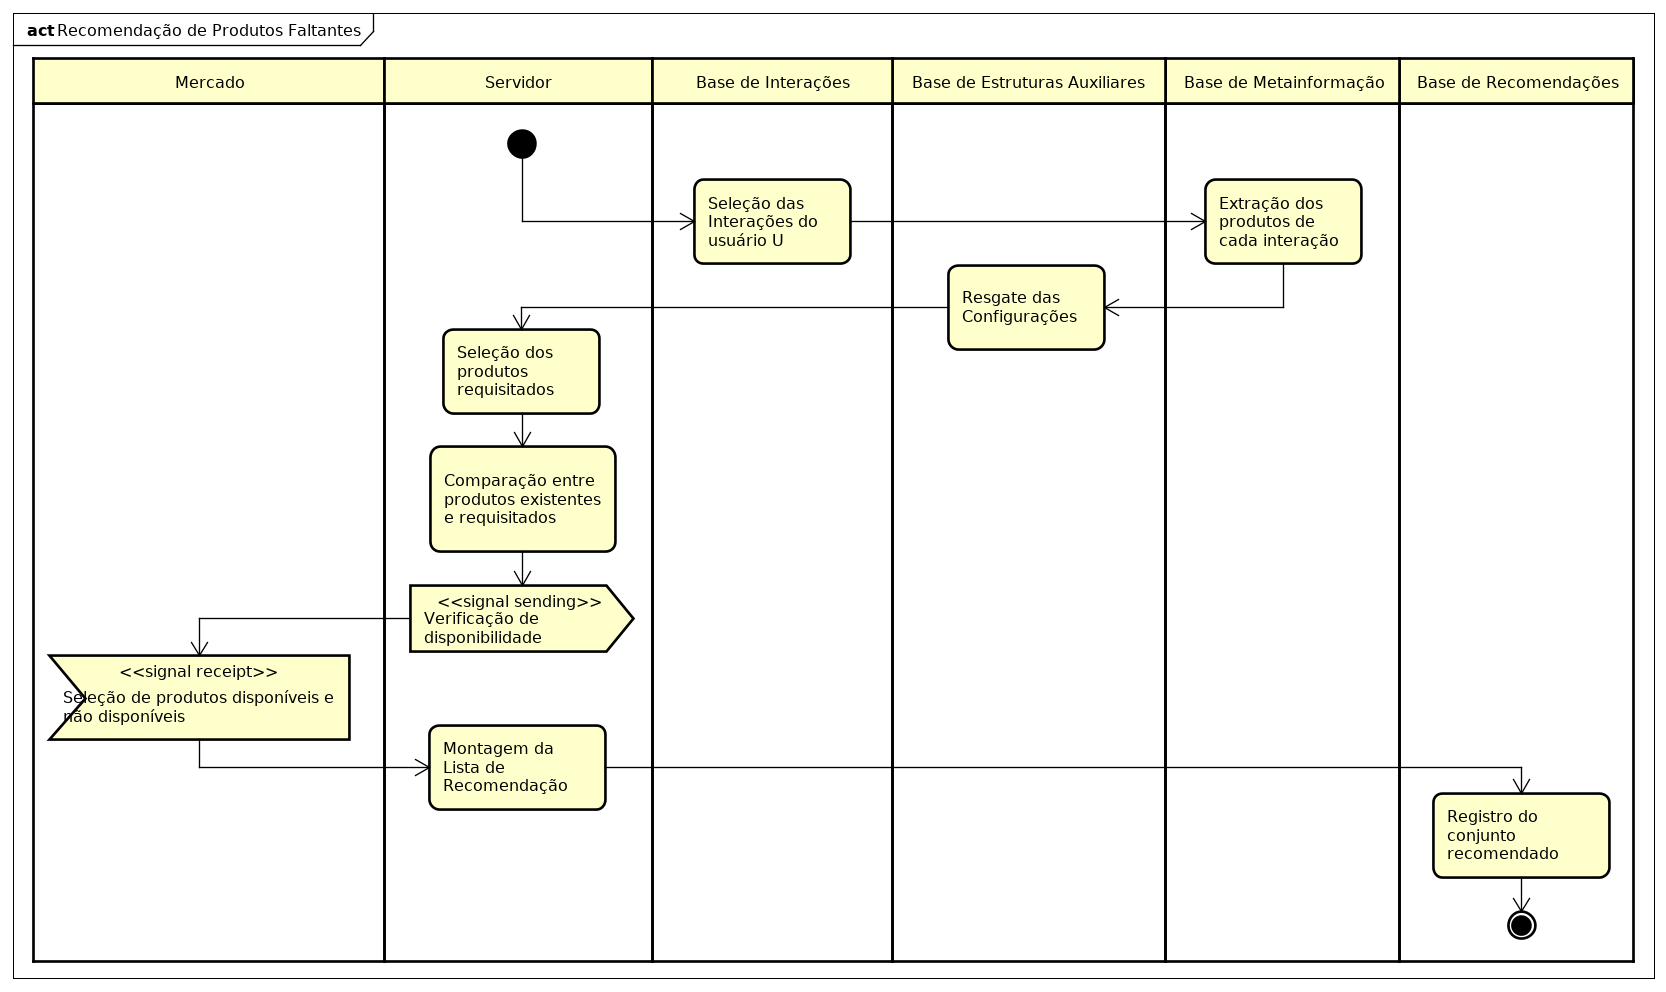
\includegraphics[width=\textwidth]{cap5_rec_produto_faltante}
    
    \footnotesize{Fonte: Elaborado pelo Autor}
\end{figure}

%%%%%%%%%%%%%%%%%%%%%%%%%%%%%%%%%%%%%%%%%%%%%%%%%%%%%%%%%%%%%%%%%%%%%%%%%
\subsection{Recomendação de Receitas por Conteúdo}

O processo de recomendação, conforme descrito na Seção \ref{sssec:proc_ger_rec}, decorre a partir da recomendação de receitas que contenham alguns dos produtos disponíveis na geladeira. 

O processo é iniciado automaticamente no servidor e o primeiro passo ocorre por meio na seleção da última interação, contendo os códigos EPC, na respectiva base de dados.

A partir dos códigos EPC, obtém-se o conjunto de produtos correspondentes a ele considerando a base de metainformação. Então, seleciona-se na base de metainformação as receitas que contenham pelo menos um dos produtos do conjunto. A partir do número de correspondências entre produtos da lista selecionada e da receita o conjunto de receitas é ordenado em ordem descendente, ou seja, receitas com maior número de correspondências primeiro. Por fim, o conjunto gerado é registrado na base de recomendações.

\begin{figure}[H]
    \caption{Fluxo para recomendação de receitas por conteúdo} 
    \label{fig:cap5_rec_receita_conteudo}
    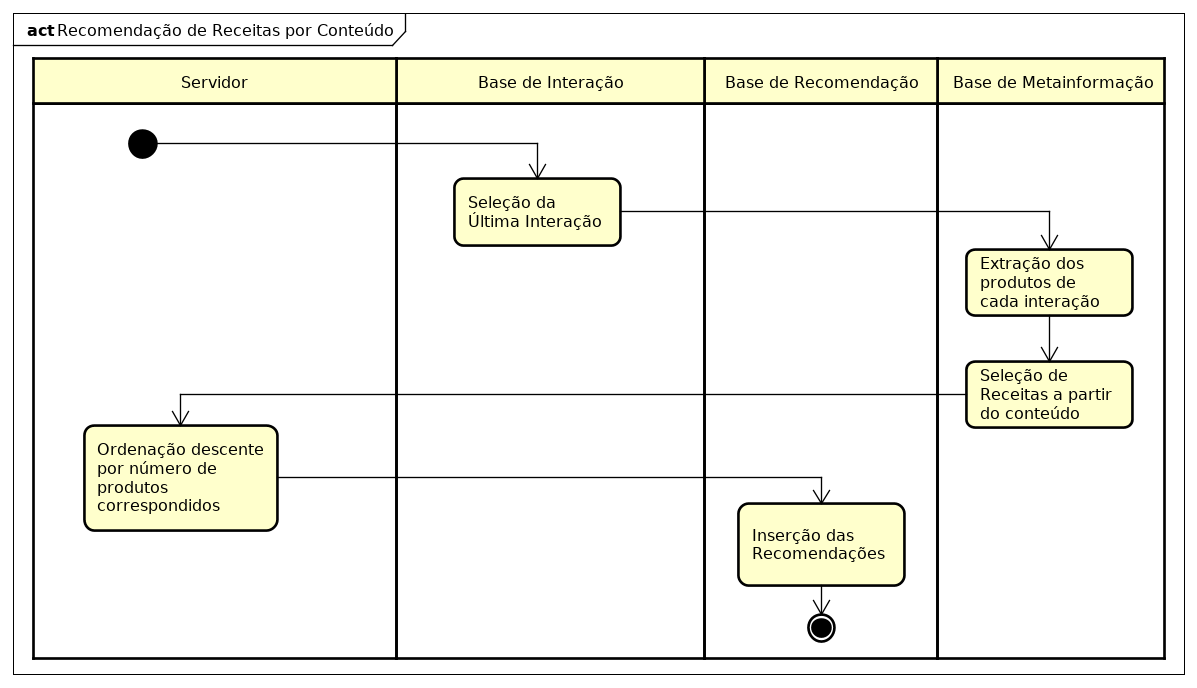
\includegraphics[width=\textwidth]{cap5_rec_receita_conteudo}
    
    \footnotesize{Fonte: Elaborado pelo Autor}
\end{figure}

%%%%%%%%%%%%%%%%%%%%%%%%%%%%%%%%%%%%%%%%%%%%%%%%%%%%%%%%%%%%%%%%%%%%%%%%%
\subsection{Recomendação de Receitas por Perfil}

A sugestão de receitas por perfil, conforme Figura \ref{fig:cap_diagr_receita_perfil}, considera os produtos com os quais o usuário mais interagiu durante a escolha de quais receitas recomendar. 

E, como nos demais processos, inicia-se no servidor automaticamente. 
O primeiro passo consiste na seleção de todas as interações do usuário na base de interações, seguida pela extração dos produtos de cada interação na base de metainformação. A partir disso, a matriz de frequências é criada e preenchida com base nos obtidos e da quantidade de vezes em que aparecem nas interações. O próximo passo, portanto, é a ordenação descendente através da frequência. Os produtos com maior frequência serão, então, utilizados como base na seleção de receitas. Nessa implementação, limitou-se em cinco (5) o número de produtos utilizados.

Com a lista de produtos, obtém-se o conjunto de receitas que contêm pelo menos um desses itens. O próximo passo consiste em ordenar a lista em disposição descendente a partir do número de produtos na receita correspondidos na lista de produtos.

Por fim, o conjunto de receitas sugeridas é registrado na base de recomendações.

\begin{figure}[H]
    \caption{Fluxo para recomendação de receitas por perfil} 
    \label{fig:cap_diagr_receita_perfil}
    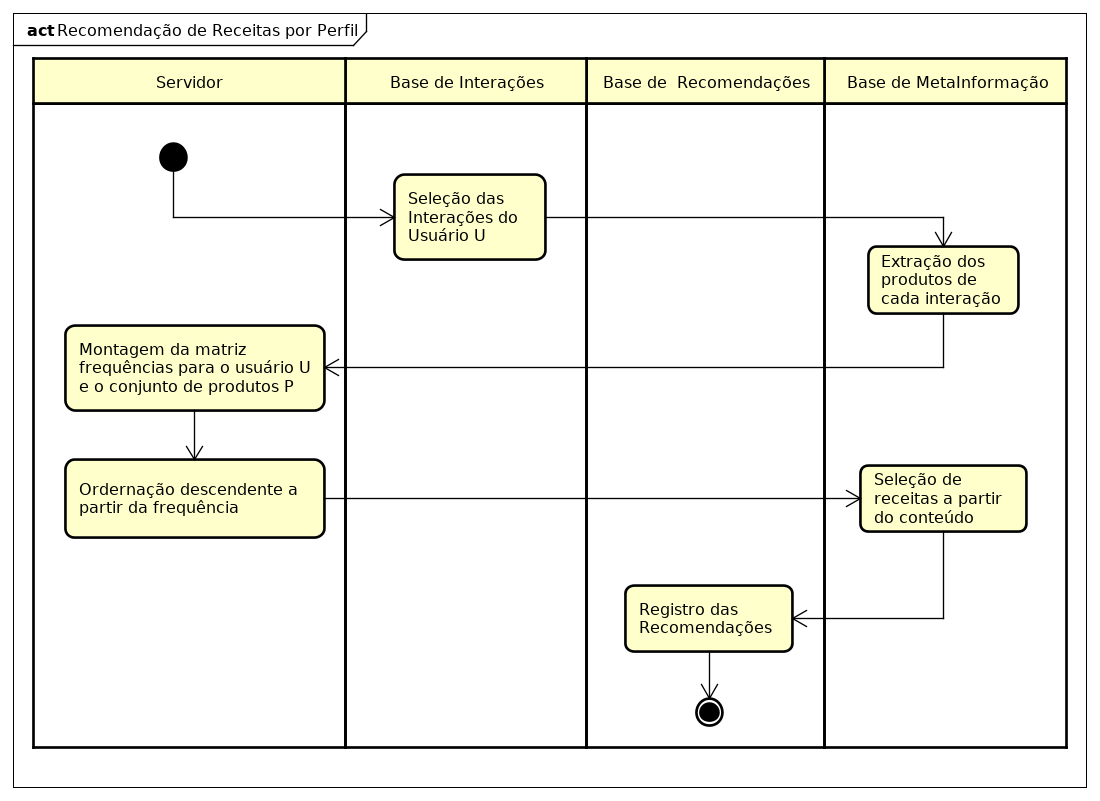
\includegraphics[width=\textwidth]{cap_diagr_receita_perfil}
    
    \footnotesize{Fonte: Elaborado pelo Autor}
\end{figure}

%%%%%%%%%%%%%%%%%%%%%%%%%%%%%%%%%%%%%%%%%%%%%%%%%%%%%%%%%%%%%%%%%%%%%%%%%
\subsection{Fluxo para Detecção e Registro de Porta Aberta}

Considerando-se, inicialmente, que a geladeira se encontra fechada. Em uma dado momento, o usuário abre-a e insere e/ou retira produtos, podendo, ao final, não fechar a porta. No momento da abertura, o sistema da geladeira detecta a ação e inicia um período de espera. Ao final desse tempo, um registro correspondente ao estado da porta é inserido na base de estruturas auxiliares.

Com relação à consulta de estado da porta, apesar de seu respectivo diagrama não ser apresentado neste trabalho, o fluxo é muito semelhante aos relacionados à consulta de listagem de produtos. Assim, quando a interface de usuário solicita o estado atual no servidor receberá o último registro realizado. A partir dele, caso indique estado aberto, uma notificação é emitida na interface.

\begin{figure}[H]
    \caption{Detecção de porta aberta}
    \label{fig:cap5_diagr_porta_aberta}
    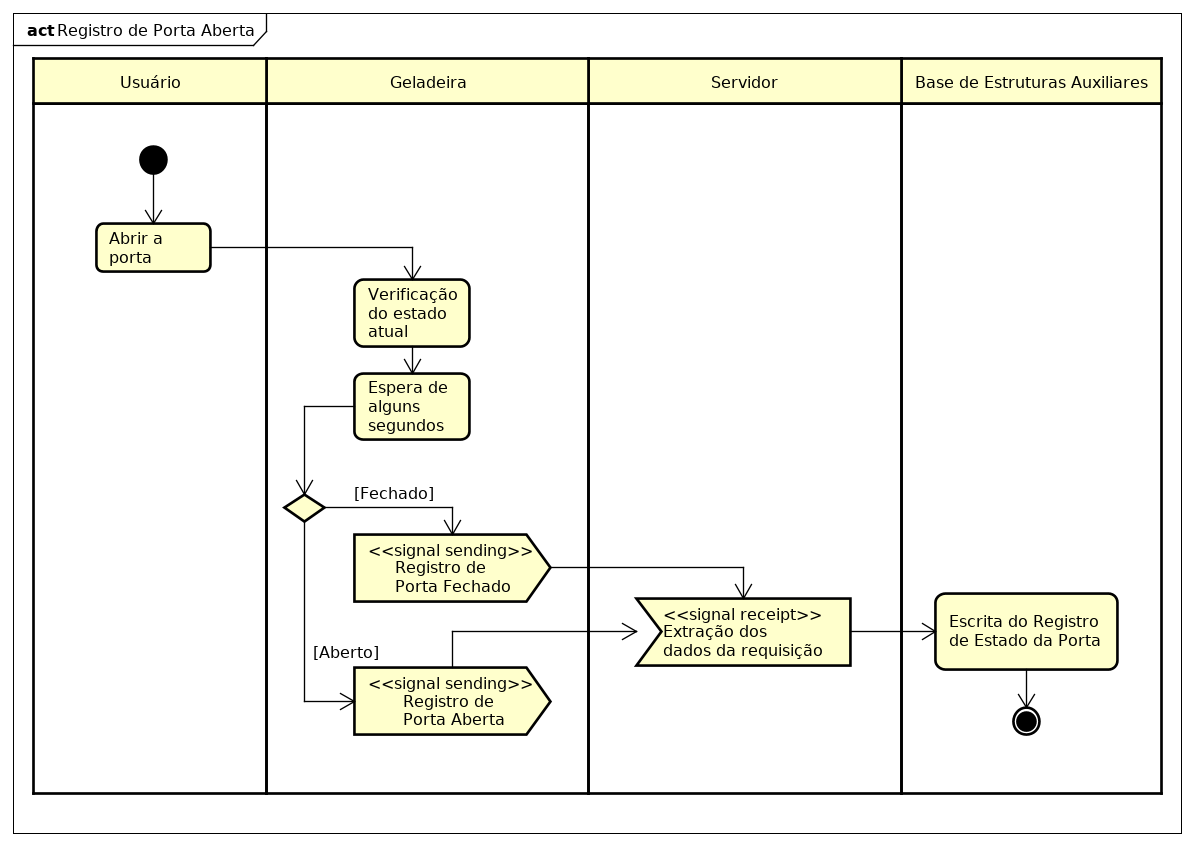
\includegraphics[width=\textwidth]{cap5_diagr_porta_aberta}
    
    \footnotesize{Fonte: Elaborado pelo Autor}
\end{figure}

\subsection{Listagem de Recomendações} \label{ssec:listagem_rec}

O processo de listagem de recomendações é disparado através da interface de usuário. Desse modo, a interface envia uma requisição ao servidor solicitando um conjunto de recomendações para um determinado usuário, conforme Figura \ref{fig:cap5_diagr_lista_rec}.  Ao receber a solicitação, o servidor faz uma busca na base de recomendações pelos produtos recomendados. Em seguida, os dados são organizados e o conjunto de recomendação é enviado à interface.

% Demonstrar fluxo de execução de listagem de recomendação
\begin{figure}[H]
    \caption{Fluxo para listagem de recomendações}
    \label{fig:cap5_diagr_lista_rec}
    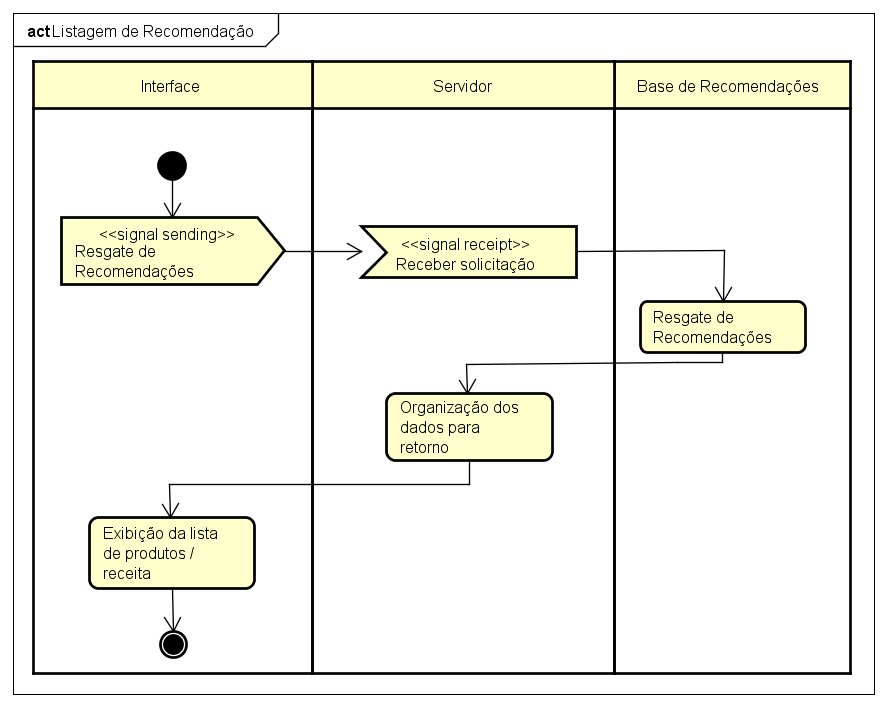
\includegraphics[width=\textwidth]{diagramas/diagr_list_rec.png}
    
    \footnotesize{Fonte: Elaborado pelo Autor}
\end{figure}

% Demonstrar fluxo de execução de listagem de produtos

\section{Cenário de Aplicação}

A avaliação do modelo dar-se-á a partir do ambiente ilustrado na Figura \ref{fig:cap5_ambiente-cenario}. O ambiente consiste na demonstração de uma sequência de ações, começando pela interação do usuário, com o objetivo de observar o comportamento e as funcionalidades do protótipo implementado.

\begin{figure}[htb]
    \caption{Ambiente do cenário}
    \label{fig:cap5_ambiente-cenario}
    \includegraphics[width=\textwidth]{figuras/cap5_cenario.png}
    
    \footnotesize{Fonte: Elaborado pelo Autor}
\end{figure}

Em relação, as bases de dados, essas foram preenchidas antes da avaliação do sistema. 
% Descrição dos dados de produtos
Primeiramente, para a base de metainformação foram alocadas informações de quarenta (40) produtos, extraídas de produtos originais a partir de um supermercado na cidade de Araranguá. Por outro lado, a informação referente à URL da imagem do produto foi obtida em \textit{websites} de supermercados.
%Excetua-se apenas o endereço URL da imagem de cada produto ao qual foi obtido \textit{websites} de supermercados. 
% Descrição de dados de receitas
Já em relação às receitas, utilizou-se dez (10) receitas obtidas a partir de sites de culinária. Tanto as informações de produtos quanto as receitas foram formatadas conforme a Seção \ref{sssec:metainfo}.

% Descrição da quantidade de usuários
Quanto à identificação das geladeiras e, por consequência, dos usuários, não criou-se uma base específica para eles, apenas atribuiu-se um identificador utilizado em cada registro específico a um determinado usuário. Como foram definidas dez (10) geladeiras, foram atribuídos os valores de um (1) a dez (10) para diferenciação de cada uma.

% Descrição da quantidade de interações por usuários.
Para cada geladeira, foram criadas, de maneira aleatória, interações, cada qual com um conjunto de códigos EPCs representando os produtos. Assim, definiu-se que o número de interações seria maior ou igual a cinco (5) e menor ou igual a 25. Além disso, para cada interação o número mínimo de itens registrados seria de três (3) e, no máximo, dez (10).

% Configurações de produtos
Em relação às configurações, descritas na Seção \ref{sssec:base_est-aux}, todas as geladeiras apresentaram parâmetros idênticos excetuando-se as listas de produtos essenciais e suas respectivas quantidades mínimas. Assim, tais produtos e suas respectivas quantidades foram definidos randomicamente para cada usuário.
%Assim, quais produtos e quais quantidades foram definidas randomicamente. 
Quanto à quantidade de produtos requisitados, estabeleceu-se o número de cinco (5) produtos e, em relação à quantidade, definiu-se um valor randômico entre um (1) e vinte (20).

% Quais os produtos que têm RFID que serão usados na geladeira
Como forma de teste do protótipo referente à estrutura física da geladeira, dois produtos receberam etiquetas com o respectivo código EPC, sendo eles, a ``Margarina com Sal Qualy\textsuperscript{\textregistered}\footnote{http://qualy.com.br/}'' e ``Creme de Leite Tirol\textsuperscript{\textregistered}\footnote{http://www.tirol.com.br/pt/}''.

%%%%%%%%%%%%%%%%%%%%%%%%%%%%%%%%%%%%%%%%%%%%%%%%%%%%%%%%%%%%%%%%%%%%%%%%%%%%%%%%%%%%%%%%%%%%%%%%%%%%%%%%%%%%%%%%%%%%%%%%%%%%%%%%%%%%%%%%%%%%%%%%%%%%%%%%%%%%%%%%%%%%%%%%%%%%%%%%%%%%%%%%%%%%%%%%%%%%%%%%%%%%%%%%%%%%%%%%%%%%%%%%%%%%%%%%%%%%%%%%%%%%%%%%%%%%%%%%%%%%%%%
\section{Avaliação do Protótipo}

Nessa seção é descrita a avaliação do protótipo criado. Para tanto, este será aplicados aos fluxos desenvolvidos na Seção \ref{sec:fluxos-de-execucao}. Assim, para cada fluxo comparar-se-á os resultados obtidos com os esperados.

%<<Descrever aqui uma introdução para esta seção>>

\subsection{Leitura do Conteúdo}
 Inicialmente a geladeira está vazia.
 Ao adicionar dois produtos, sendo eles, a ``Margarina com Sal Qualy\textsuperscript{\textregistered}'' e ``Creme de Leite Tirol\textsuperscript{\textregistered}'', respectivamente, depois de alguns minutos os seguintes códigos EPC são lidos.
 
\begin{itemize}[noitemsep,topsep=5pt]
     \item 8665580279609348107299713701
     \item 8665580277303506451141610373
 \end{itemize}
 
 Os dados são, então, enviados ao serviço de registro de interação e o registro é gravado na base de interações, conforme apresentado no Quadro \ref{fig:cap5_registro_interacao}. 
 
 %%%%%%%% JSON DO REGISTRO  %%%%%%%%
 \begin{quadro}[htb]
     \caption{Registro de interação dos produtos}
     \label{fig:cap5_registro_interacao}
     
     \frame{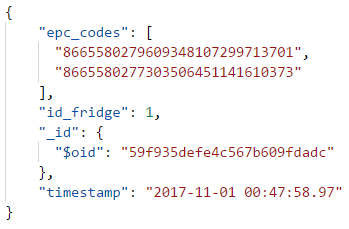
\includegraphics[width=0.5\textwidth]{cap5_registro_interacao}}
     
     \footnotesize{Fonte: Elaborado pelo Autor}
 \end{quadro}
 
\subsection{Listagem de Conteúdo da Geladeira}
 
Continuando o fluxo da seção anterior, ao tentar ler o conteúdo da geladeira logo após o fechamento da porta, a listagem da interface ainda se mantém vazia. Alguns segundos depois, a listagem é atualizada e o conteúdo exibido é mostrado na Figura \ref{fig:cap5_listagem_atual}.


 %%%%%%%%%%%%%%%%%%%%%   FIGURA DA LISTAGEM APÓS A INTERAÇÃO %%%%%%%%%%%%%%%%%%%%%%%%%%%%%%%%%%%
\begin{figure}[htb]
    \caption{Listagem de produtos na Interface}
    \label{fig:cap5_listagem_atual}
    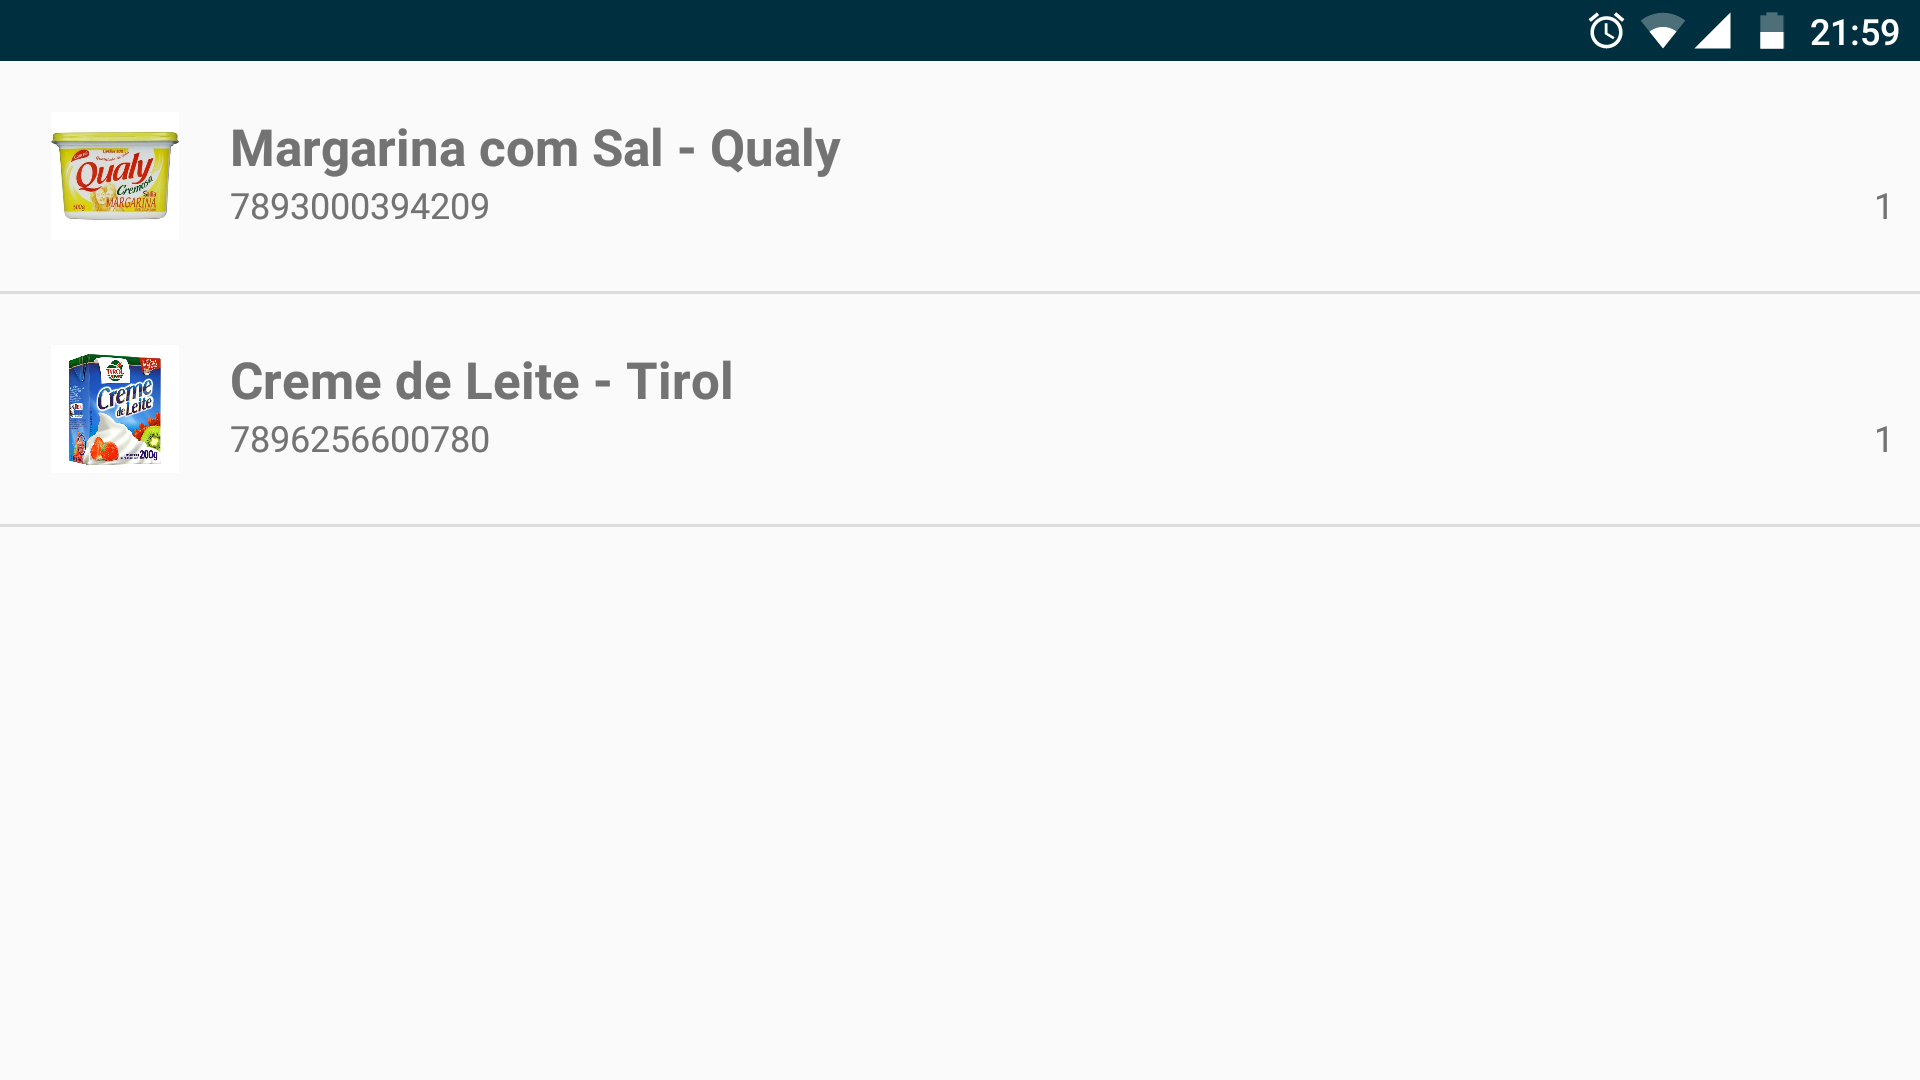
\includegraphics[width=0.8\textwidth]{cap5_listagem_atual}
    
    \footnotesize{Fonte: Elaborado pelo Autor}
\end{figure}
 
Dessa forma, afirma-se que a listagem de produtos produz resultados de acordo com o esperado, já que a lista é alterada após a interação. No entanto, o fator temporal entre a interação e a exibição é compreensível. Assim, o intervalo de tempo decorre do aguardo, na geladeira, até a realização da leitura. Isso é necessário para garantir que exista tempo hábil para coletar ou inserir todos os produtos que se deseja.


%%%%%%%%%%%%%%%%%%%%%%%%%%%%%%%%%%%%%%%%%%%%%%%%%%%%%%%%%%%%%%%%%%%%%%%%%%%%%%%%%%%%%%%%%%%%%%
\subsection{Recomendações de Produtos Novos}

Como exemplo, deseja-se gerar recomendações para o Usuário 1. Para tanto, seguiu-se o fluxo da Seção \ref{ssec:geracao_rec_novo}. Os passos foram executados até o cálculo de similaridade entre usuários sobre a matriz de frequências de interações e obteve-se o usuário mais semelhante. Tal indivíduo é identificado como Usuário 10 e o grau de similaridade entre este e o Usuário 1 foi de 0,15. A média de interações com produtos para o Usuário 1 foi de 2,05, já para o Usuário 10 foi de 2,12.

%inicia-se com a criação da matriz de frequências seguida pelo resgate das interações e, a partir dessas, dos códigos de barras e, por fim o preenchimento da matriz, conforme Figura \ref{fig:cap5_diagr_geracao_rec}.

Como forma de verificação, conforme Tabela \ref{tab:cap5_matriz_sim}, tem-se as linhas da matriz de frequência referentes aos usuários.


%%%%%%%%%%%%%%%%%%  MATRIZ  %%%%%%%%%%%%%%%%%%%%%%
\begin{table}[htb]
\caption{Matriz de frequências de interações}
\label{tab:cap5_matriz_sim}
%\begin{tabular}{C{0.72cm}c}
\toprule
\textbf{U1} \hspace{0.23cm} 0 2  2  6  2  3  6  0  2  4  2  5  2  1  1  2  1  8  5  6  5  1  2  3  3  5  5  3  1  0  0  0  0  0  0 \vspace{0.1cm} \midrule 
\textbf{U10} \hspace{0.02cm} 2  2  7  3  3  3  4  3  0  0  2  4  0  0  4  0  2  9  6  0  2  0  0  5  4  0  2  3  1  2  4  7  5  2  3 \vspace{0.1cm}  \bottomrule \vspace{0.1cm} 
%\end{tabular}

\footnotesize{Fonte: Elaborado pelo Autor}
\end{table}        

\newpage
Executando o cálculo da correlação de Pearson, descrita na Equação \ref{eq:correlacao-pearson}.

%%%%%%%%%%%%%%%%%%  EQUAÇÃO COM VALORES SUBSTITUÍDOS  %%%%%%%%%%%%%%%%%%%%%%%%%%%%%%
\begin{equation}
sim=\dfrac{\left[
\splitdfrac{
(0-2,05)(2-2,12)+
(2-2,05)(2-2,12)+
}
{\splitdfrac{
(2-2,05)(7-2,12)+
(6-2,05)(3-2,12)+
}{
(2-2,05)(3-2,12)+...}}\right]}
{
\left[
\splitdfrac{
\sqrt{\splitdfrac{(0-2,05)^2+
(2-2,05)^2+
(2-2,05)^2+
}{
(6-2,05)^2+
(2-2,05)^2+...}}
}{
\times\sqrt{\splitdfrac{(2-2,12)^2+
(2-2,12)^2+}{\splitdfrac{
(7-2,12)^2+
(3-2,12)^2+
}{
(3-2,12)^2+...}}}
}\right]
}
\nonumber
\end{equation}

\begin{equation}
sim = 0,15 \nonumber
\end{equation}

Assim, demonstra-se que o cálculo de similaridade está correto. Percebe-se que o número de produtos com os quais o Usuário 1 não apresentou nenhuma interação, ou seja, as posições na linha do usuário mencionado preenchidas com zero (0) é igual a oito (8). Assim, espera-se que pelos menos esses produtos sejam recomendados.

No entanto, um número maior de itens podem ser sugeridos. Isso ocorrerá quando a quantidade obtida de recomendações através do usuário com maior similaridade for insuficiente. Assim, recomendações de outros usuários com graus de semelhança menores serão consideradas.

Obteve-se, a partir da consulta à base de recomendações, a seguinte lista de itens:

\begin{itemize}[noitemsep,topsep=5pt]
%    \item 7892840800000 - Refrigerante Pepsi
    \item 789034630442 - Creme de Leite Parmalat
    \item 7894900093056 - Iogurte Danone
    \item 7896648699453 - Leite Integral Langaru
    \item 7894904326044 - Pizza Calabresa Seara
%    \item 7891991010481 - Cerveja Budweiser
    \item 7896256603422 - Leite Desnatado Tirol
    \item 7896256602050 - Iogurte de Morango Tirol
    \item 7891025101376 - Iogurte Danone
    \item 7896034680010 - Leite Condensado Parmalat
    \item 7891515490430 - Lasanha Calabresa Perdigão
\end{itemize}

 %%%%%%%%%%%%%%%%%%%%%   FIGURA DA LISTAGEM DE RECOMENDAÇÕES DE PRODUTOS NOVOS %%%%%%%%%%%%%%%%%%%%%%%%%%%%%%%%%%%

Os primeiros oito produtos da lista são aqueles que o Usuário 1 não interagiu, mas que o Usuário 10 o fez, na mesma sequência mostrada na Tabela \ref{tab:cap5_matriz_sim}. Já os demais itens foram sugeridos com base em outros usuários com menor similaridade. Vale ressaltar que o JSON gerado pelo sistema não foi inserido diretamente neste trabalho visto a extensão do mesmo.

\subsection{Recomendação de Produtos Faltantes}

Nesta seção, busca-se avaliar a recomendação da reposição de produtos aos quais o Usuário 2 julga serem essenciais. Para tanto, considera-se o fluxo de execução demonstrado na Seção \ref{ssec:cap5_rec_prod_falt} e o conjunto de produtos contidos atualmente e suas respectivas quantidades:

%%%%%%%%%%%%%%% Lista de um conjunto de produtos atuais %%%%%%%%%%%%%%%
\begin{itemize}[noitemsep,topsep=5pt]
    \item Mortadela Perdigão\textsuperscript{\textregistered} \footnote{http://www.perdigao.com.br/} 5 UN
    \item Pizza Calabresa Sadia\textsuperscript{\textregistered} \footnote{http://www.sadia.com.br/}, 4 UN
    \item Iogurte de Morango Activia\textsuperscript{\textregistered}\footnote{https://www.activiadanone.com.br/}, 5 UN
\end{itemize}

E o conjunto de produtos que o Usuário 2 estipulou que sempre devem estar à disposição:

%%%%%%%%%%%%%%% Lista de um conjunto de produtos essenciais %%%%%%%%%%%%%%%
\begin{itemize}[noitemsep,topsep=5pt]
    \item Mortadela, 8 UN
    \item Pizza Calabresa, 6 UN
    \item Iogurte de Morango, 5 UN
    \item Linguiça de Pernil, 15 UN
    \item Leite integral, 8 UN
\end{itemize}


Percebe-se que alguns produtos estão ausentes e, outros, em falta como, por exemplo, o produto Pizza está em quantidade insuficiente e o produto Leite está ausente. Assim, a recomendação deve conter tais produtos além dos outros não citados.

Seguindo o fluxo da Seção \ref{ssec:listagem_rec}, tem-se a listagem de sugestões na interface de usuário como é mostrado na Figura \ref{fig:cap5_rec_faltante}.

\begin{figure}[htb]
    \caption{Listagem de Recomendações por falta}
    \label{fig:cap5_rec_faltante}
    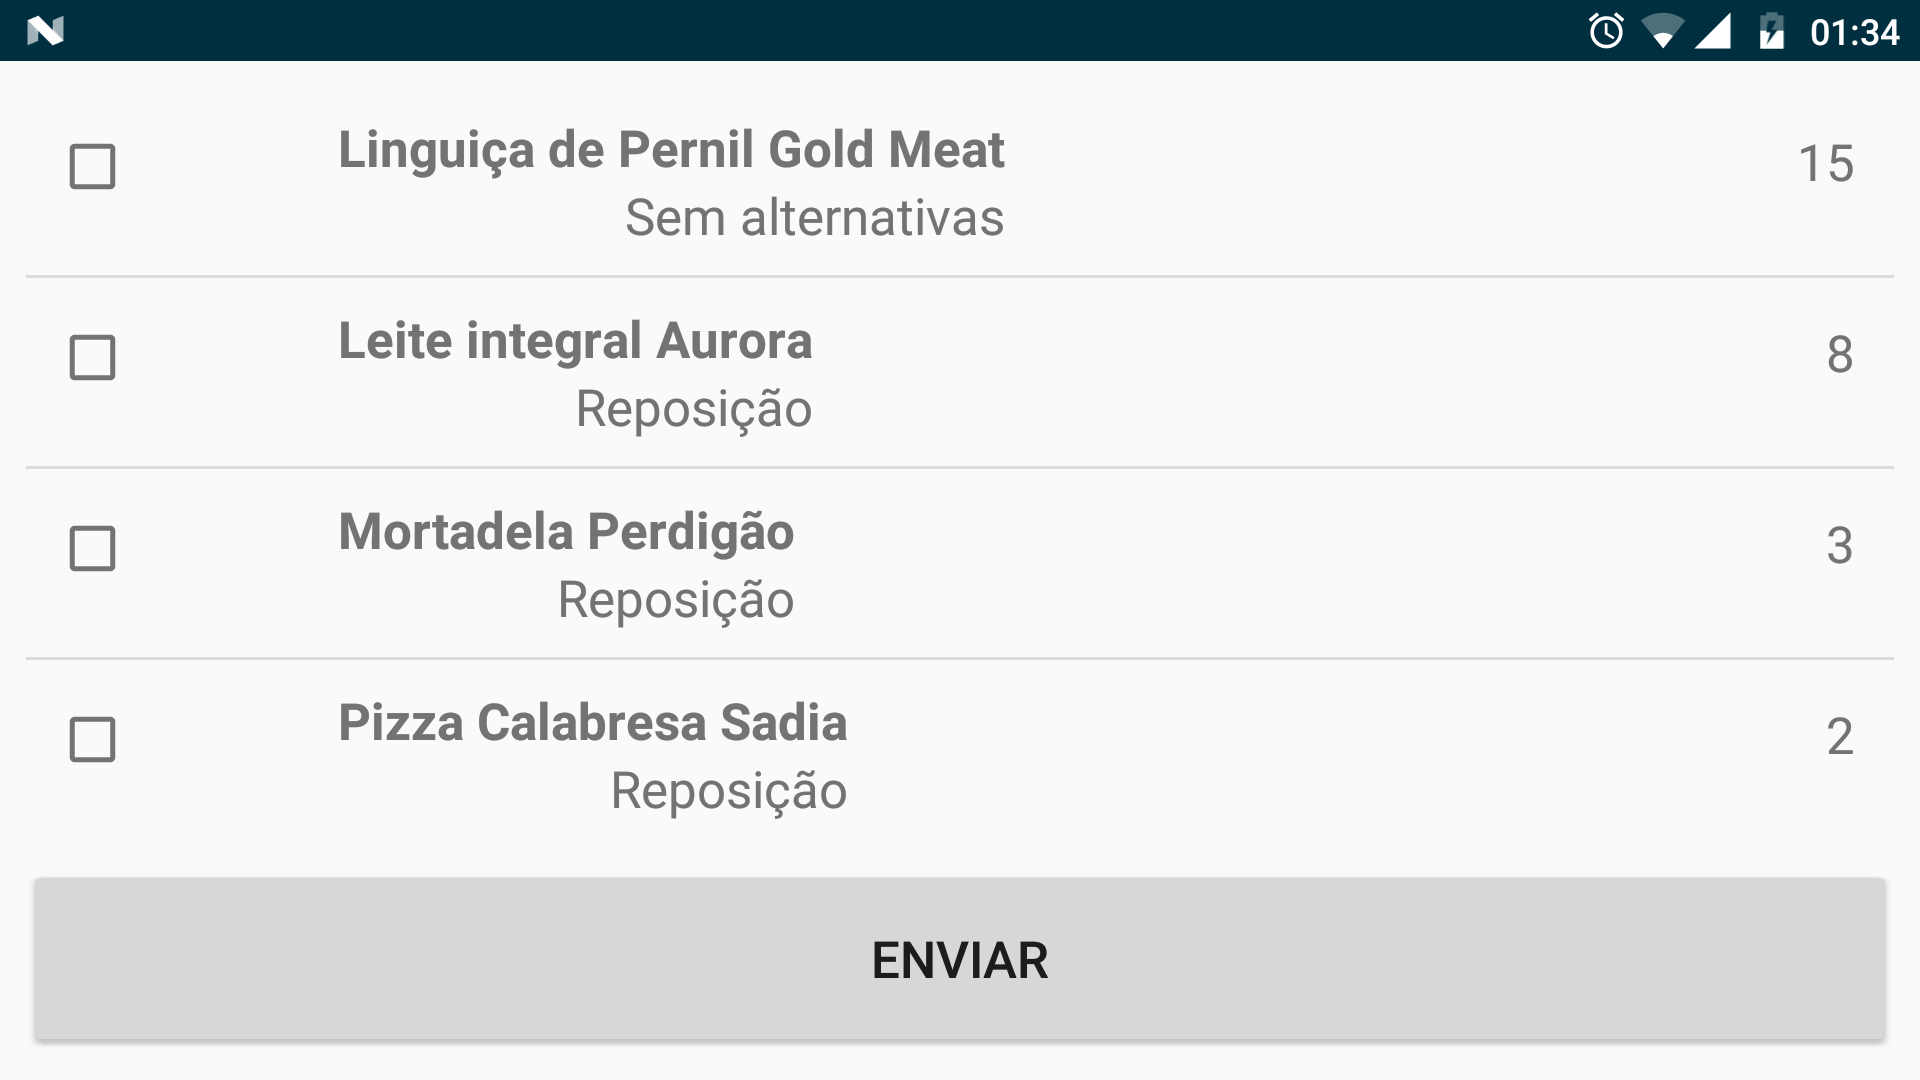
\includegraphics[width=0.8\textwidth]{cap5_rec_faltante}
    
    \footnotesize{Fonte: Elaborado pelo Autor}
\end{figure}

%%%%%%%%%%%%%%% Lista de um conjunto de produtos recomendados %%%%%%%%%%%%%%%

Pode-se verificar que há diferenciação entre os produtos, sendo de ``Reposição'' e ``Sem Alternativas''. A reposição trata da recolocação de produtos essenciais. O ``Sem alternativas'', indica que não foi possível encontrar no mercado, o produto esperado nem um similar a ele. Há, além disso, outras duas formas de recomendação de compras: ``Novo'', referente à recomendação de produtos novos, como descrito anteriormente, além de ``Similar'' que indica a reposição de produtos essenciais que não estavam disponíveis no mercado, mas que foram substituídos por produtos similares.

\subsection{Recomendação de Receitas a partir de Conteúdo}

A recomendação de receitas por conteúdo, como descrito na seção respectiva no Capítulo 4, busca disponibilizar um conjunto de receitas ao usuário de acordo com os itens que este possui em sua geladeira. 

Considera-se que, inicialmente, os seguintes produtos estejam disponíveis com suas respectivas quantidades:

\begin{itemize}[noitemsep,topsep=5pt]
    \item Leite Integral, com 2 UN
    \item Leite Condensado Parmalat\textsuperscript{\textregistered}\footnote{http://www.parmalat.com.br/}, com 3 UN 
    \item Queijo Mussarela Sadia\textsuperscript{\textregistered}, com 5 UN.
\end{itemize}

O processo de recomendação avaliará os produtos do ponto de vista de suas características, ou seja, terá um enfoque nos tipos de produtos e não em produtos de determinadas marcas.

O processo de recomendação analisa quais receitas satisfazem o requisito especificado e retornará um conjunto de itens como sugestão.

Os itens sugeridos como recomendações são mostrados na Figura \ref{fig:cap5_rec_recipe_content}.

%%%%%%%%%%%%%%%%%%    FIGURA X (Lista de receitas de recomendação)    %%%%%%%%%%%%%%%%%%%%%%%%%%%%%
\begin{figure}[htb]
\caption{Resultado da recomendação de receitas}
\label{fig:cap5_rec_recipe_content}
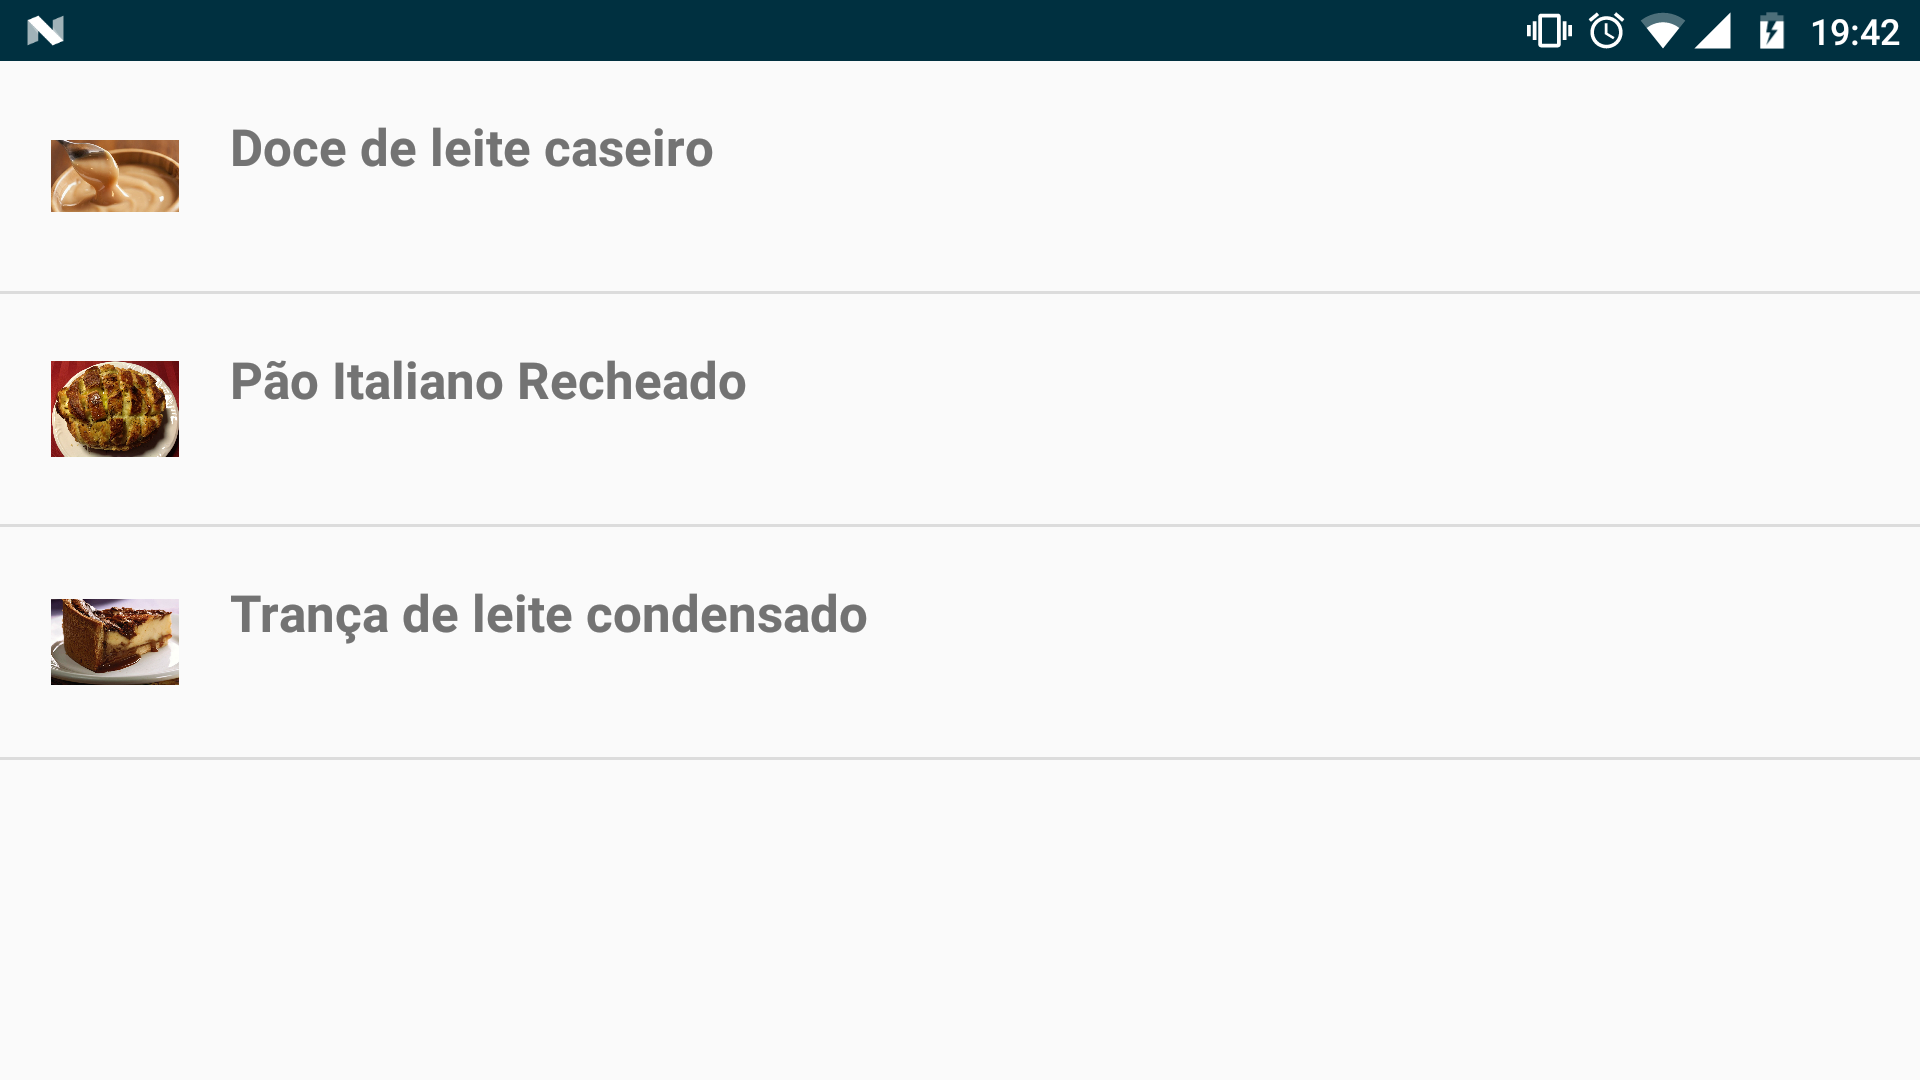
\includegraphics[width=0.8\textwidth]{cap5_rec_recipe_content}

\footnotesize{Fonte: Elaborado pelo Autor}
\end{figure}

Como resultado da recomendação, tem-se três receitas sugeridas dentre as cinco utilizadas nesse cenário, ou seja, duas receitas não incluíam nenhum dos produtos contidos na geladeira. A primeira receita na lista conta com o Leite, a segunda com o Queijo Mussarela e a terceira com Leite e Leite Condensado.

\subsection{Recomendação de Receitas por Perfil}

Como descrito na Seção \ref{sssec:proc_ger_rec}, a sugestão de receitas por perfil buscará receitas que contenham alguns dos itens com os quais o usuário mais interagiu. Para tanto, uma matriz de frequência de interações é elaborada. Com base nas frequências de interações do usuário em questão, uma lista é criada a partir das classes de produto.

Considerando que o total de produtos para geração de recomendação foi limitado em cinco (5) tem-se os seguintes produtos:

\begin{itemize}[noitemsep,topsep=5pt]
    \item Margarina com Sal Qualy, com 9 interações
    \item Refrigerante de Guaraná Fanta, com 9 interações
    \item Linguiça de Pernil Gold Meat, com 8 interações
    \item Iogurte Danone, com 7 interações
    \item Queijo Mussarela Sulfrios, com 7 interações
\end{itemize}

Com base neste conjunto, o processo de recomendação realiza uma busca na base de interações pela receitas que possuem tais categorias de produtos. A partir disso, o conjunto de receitas da Figura \ref{fig:cap5_rec_recipe_profile} foi sugerido.


%%%%%%%%%%%%%%%%%%%%%% FIGURA RECEITA SUGERIDA %%%%%%%%%%%%%%%%%%%%

\begin{figure}[htb]
    \caption{Lista de Receitas Sugeridas por Perfil}  
    \label{fig:cap5_rec_recipe_profile}
    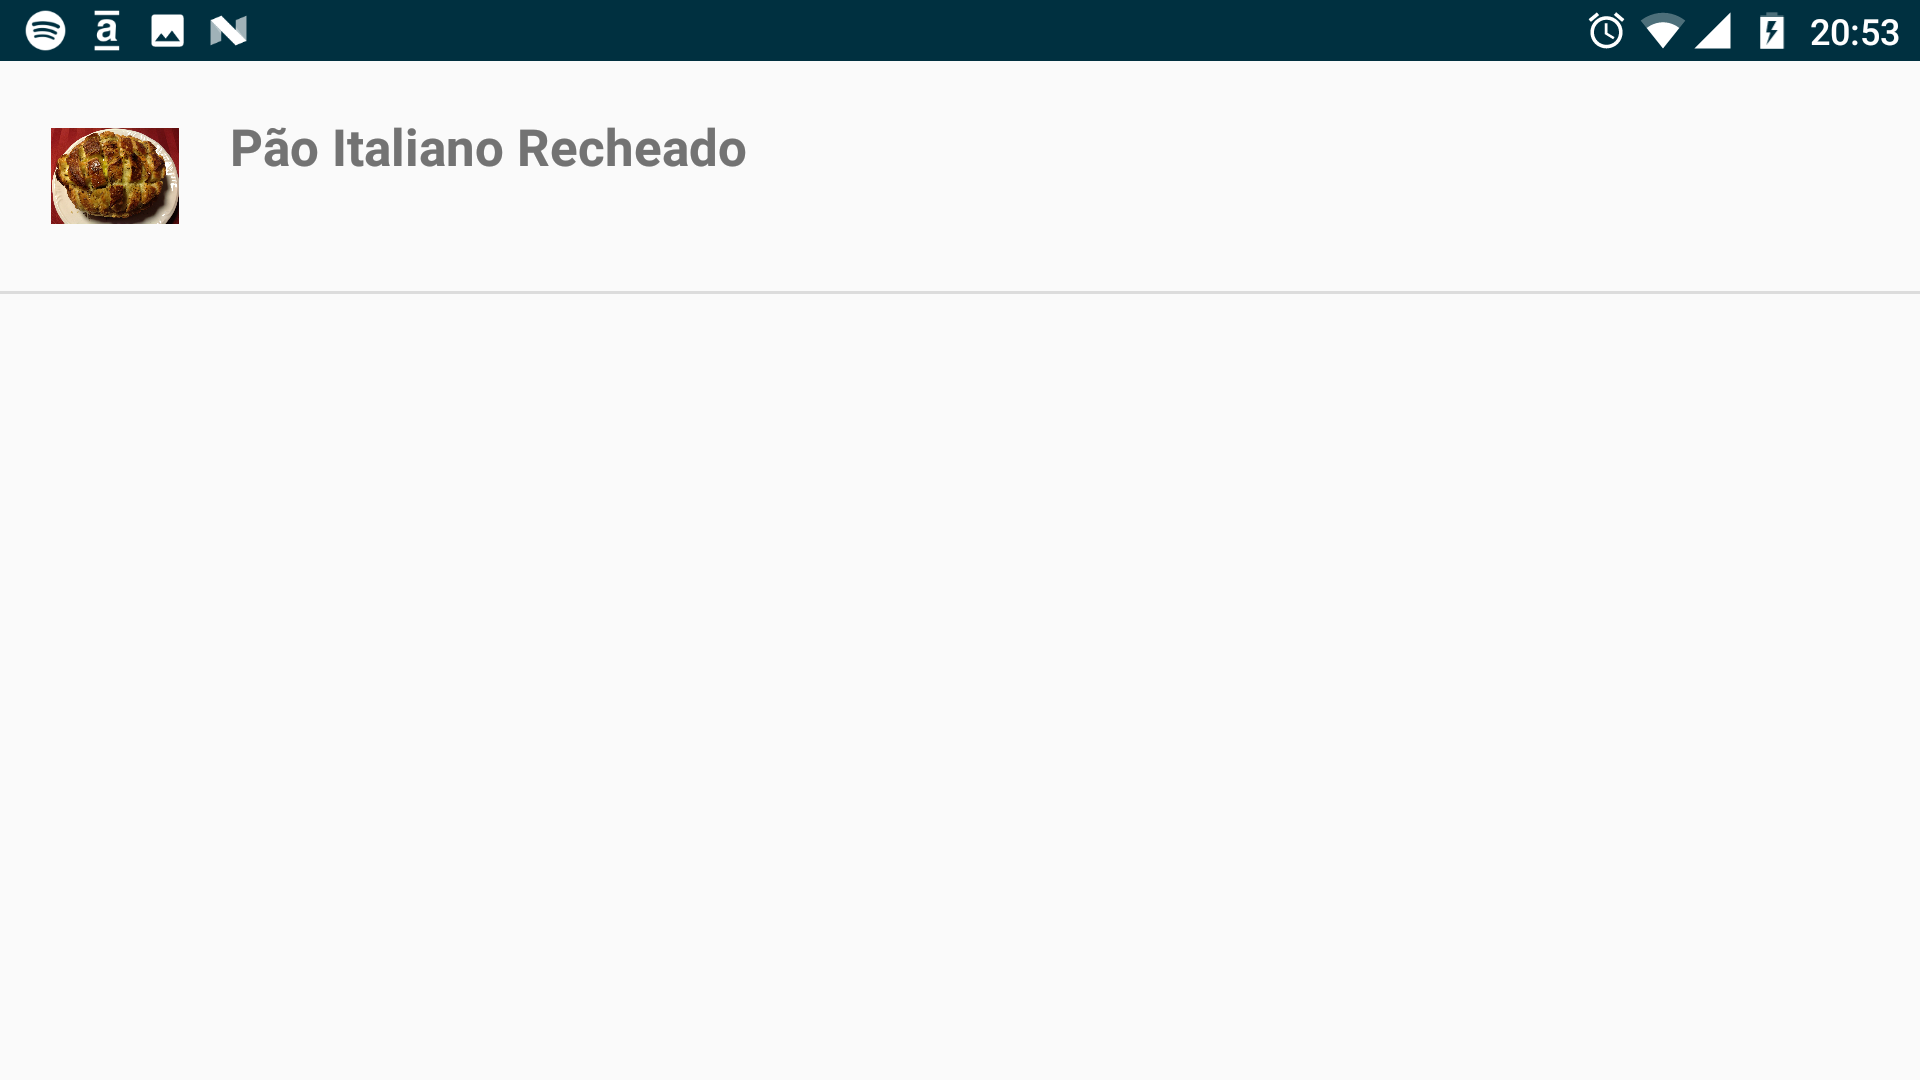
\includegraphics[width=0.8\textwidth]{cap5_rec_recipe_profile}
   
    \footnotesize{Fonte: Elaborado pelo Autor}
\end{figure}

Apesar de apenas uma receita ter sido sugerida, devido ao total de receitas muito reduzido do cenário, é possível validar a recomendação, já que esta conta com o produto Queijo Mussarela.

\subsection{Alerta de Porta Aberta}

%% OBJETIVO
Os alertas enviados aos usuários que esquecem a porta da geladeira aberta, ou não a fecham corretamente, é importante para evitar gastos desnecessários com energia e, possivelmente, com alimentos estragados. Como descrito na Seção \ref{ssec:c5_camada_servicos}, o processo de verificação de porta aberta, dispara um registro no servidor. Para o exemplo, considera-se que inicialmente a porta estava fechada e, em um dado momento, foi deixada aberta.

Após alguns segundos o registro do Quadro \ref{fig:cap5_open_door_reg} foi efetuado na base de estruturas auxiliares, informando a situação.


%%%%%%%%%%%%%%%%% REGISTRO DE PORTA ABERTA  %%%%%%%%%%%%%%%
\begin{quadro}[H]
    \caption{Registro de porta aberta}
    \label{fig:cap5_open_door_reg}
    \frame{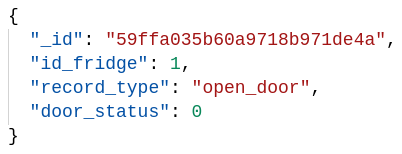
\includegraphics[width=0.5\textwidth]{cap5_open_door_reg}}
    
    \footnotesize{Fonte: Elaborado pelo Autor}
\end{quadro}

Algum tempo depois, a interface de usuário realiza uma requisição ao serviço de estado de porta. Neste caso, a aplicação da interface verificou que o estado era aberto e notificou ao usuário, conforme a Figura \ref{fig:cap5_open_door_alert}.


%%%%%%%%%%%%%%% IMG NOTIFICAÇÃO DE PORTA ABERTA  %%%%%%%%%%%%
\begin{figure}[H]
    \caption{Alerta de porta aberta}
    \label{fig:cap5_open_door_alert}
    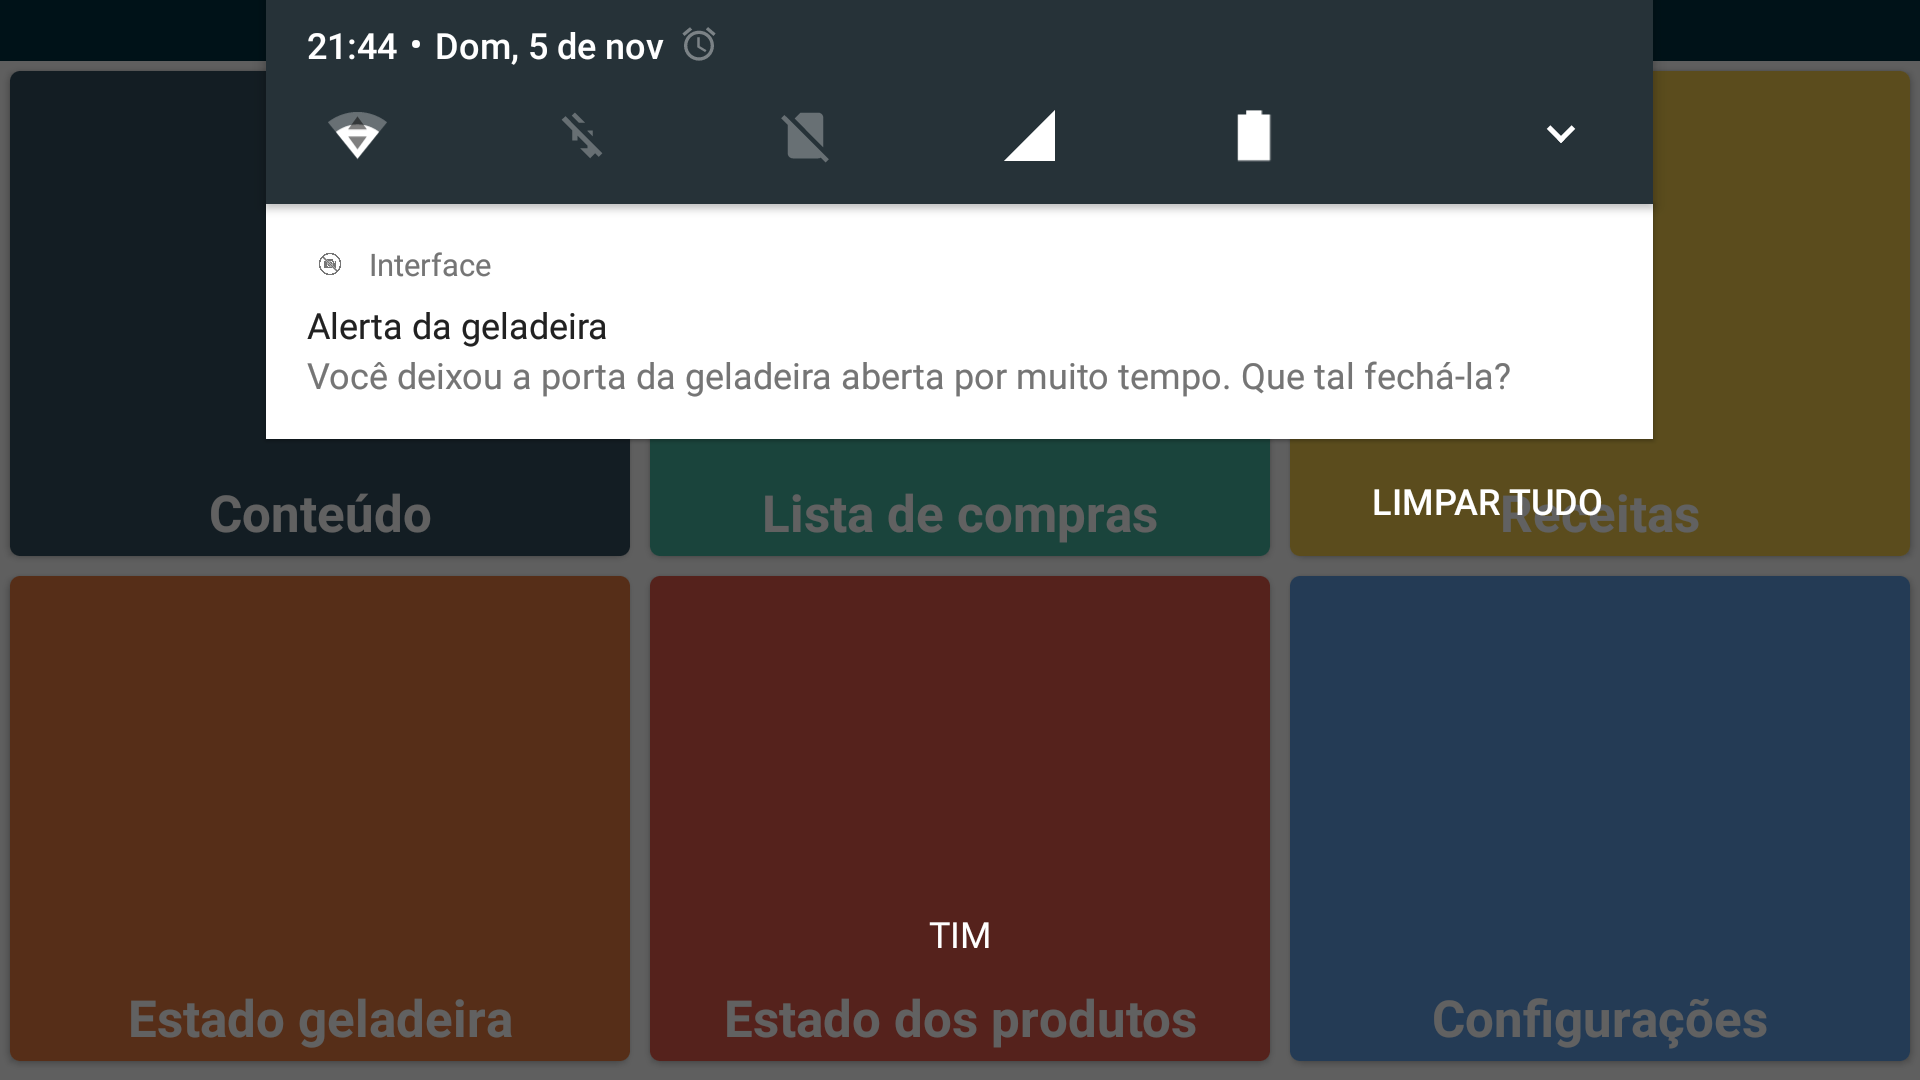
\includegraphics[width=\textwidth]{cap5_open_door_alert}
    
    \footnotesize{Fonte: Elaborado pelo Autor}
\end{figure}





	%\chapter{Considerações Finais}
\label{cap:consideracoes_finais}
\section{Conclusões}

\section{Trabalhos Futuros}

 %Visão computacional: integrar computação visual na identificação de produtos e das interações que ocorrem, ou seja, usar computação visual para 

 %Integração com a assistente pessoal Alexa, onde o Amazon Echo se torna um 'gateway' e a geladeira se comunica apenas com o Echo.

 %Uso de uma placa de leitura única, por toda a prateleira

 %Possibilidade de ser aplicado em qualquer lugar

% Substituição do Raspberry por um sistema embarcado propriamente dimensionado para o projeto e que integre com o resto do sistema e possa gerenciar melhor o consumo de energia.

% Comunicação com outros dispositivos da casa

% Recomendação mais inteligente que consiga recomendar produtos para perfis específicos como intorantes a lactose, vegetarianos a partir da configuração do usuário.
	
	%--------------------------------------------------
	
	\bibliographystyle{ufscThesis/ufsc-alf}
	\bibliography{postextual/referencias}

	%-------------------------\textsl{}-------------------------------
	% Elementos pós-textuais
	%\apendice
%\chapter{Exemplificando um Apêndice}
%Texto do Apêndice aqui. 
	%\anexo
%\chapter{Matriz de Frequências Referentes aos Usuário 1 e 10}
%Texto do anexo aqui.



\end{document}
